\documentclass[sigconf, nonacm]{acmart} %manuscript
% \documentclass[manuscript, nonacm]{acmart} 
\setcopyright{none}
%\documentclass[11pt,twoside,a4paper]{article}
%\usepackage{subfig}
\usepackage{hyperref}
\usepackage[utf8]{inputenc}

\usepackage{pgfplots}
\newtheorem{remark}{Remark}
\newtheorem{definition}{Definition}

% \usepackage{fontspec}
% \setmainfont{Garamond}


% Keywords command
%\title{MIND-BIG: Mining Dense Subgraphs in Bipartite Graphs in Parallel}
\title{Theoretically Efficient Parallel Density-Peak Clustering}
% \subtitle{PRIMES Final Research Paper \newline 
% December 31, 2021}


\author{Yihao Huang}
\affiliation{%
  \institution{Phillips Academy\\ yhuang23@andover.edu}
}


\usepackage{xy}
\usepackage{tikz}
\usepackage{mathrsfs}
\usepackage{setspace,dsfont,graphicx,makecell,appendix,multirow,float}
\pgfplotsset{compat=1.17}

\usepackage{bbm}
\usepackage{graphicx}
\usepackage{booktabs}
\usepackage{amsthm}
\usepackage{amsmath}
\usepackage{times}
\usepackage{multirow}
\usepackage{tabularx}
\usepackage{dblfloatfix}
%\usepackage{enumitem}
%\setlist{noitemsep,topsep=0pt,parsep=0pt,partopsep=0pt}
\usepackage{xspace}
%\usepackage{algorithmicx}
\usepackage{algorithm}
\usepackage[noend]{algpseudocode}
\usepackage{subcaption,graphicx,url,multicol,mathtools}
\usepackage{paralist}
\usepackage{color}
\usepackage{arydshln}
\usepackage[most]{tcolorbox}
\usepackage{stmaryrd}
\usepackage{bm}
\graphicspath{ {./figures/} }

\newcommand{\BigO}[1]{\ensuremath{O(#1)}}
\newcommand{\BigOmega}[1]{\ensuremath{\Omega(#1)}}
\newcommand{\slfrac}[2]{\left.#1\middle/#2\right.}
\newcommand{\Var}[1]{\operatorname{Var}\left[#1\right]}
\newcommand{\whp}[1]{w.h.p.}
\newcommand{\algname}[1]{\textnormal{\textsc{#1}}}


% declaration of the new block
\algblock{ParFor}{EndParFor}
% customising the new block
\algnewcommand\algorithmicparfor{\textbf{parfor}}
\algnewcommand\algorithmicpardo{\textbf{do}}
\algnewcommand\algorithmicendparfor{}%\textbf{end\ parfor}
\algrenewtext{ParFor}[1]{\algorithmicparfor\ #1\ \algorithmicpardo}
\algrenewtext{EndParFor}{\algorithmicendparfor}
\algtext*{EndParFor}

\algdef{SE}[DOWHILE]{Do}{doWhile}{\algorithmicdo}[1]{\algorithmicwhile\ #1}%

\makeatletter
\newtheorem*{rep@theorem}{\rep@title}
\newcommand{\newreptheorem}[2]{%
\newenvironment{rep#1}[1]{%
 \def\rep@title{#2 \ref{##1}}%
 \begin{rep@theorem}}%
 {\end{rep@theorem}}}
\makeatother

\newtheorem{theorem}{Theorem}
\newcommand{\myparagraph}[1]{\noindent {\bf #1.}}
\usepackage{comment}

\newcommand{\shangdi}[1]{{\color{blue}{\bf Shangdi:} #1}}
\newcommand{\michael}[1]{{\color{purple}{\bf Michael:} #1}}

\begin{document}


\begin{abstract}


\onehalfspacing
\myparagraph{Abstract}

Clustering multidimensional points is a fundamental data mining task, with applications in astronomy, neuroscience, bioinformatics, and computer vision, just to name a few. Density-based clustering is a clustering framework that defines clusters as dense regions of points. It has the advantage of being able to detect clusters of arbitrary shapes, rendering it useful in many applications. 

In this paper, we propose fast and theoretically efficient parallel algorithms for the Density-Peaks Clustering problem, a recently proposed approach for density-based clustering. DPC is effective in detecting clusters of arbitrary shapes, and is theoretically simple as it circumvents the difficulty of choosing a density threshold in classic density-based clustering approaches, such as the DBSCAN algorithm. However, existing DPC algorithms either suffer from an exorbitant quadratic runtime complexity or don't have a high degree of parallelism, limiting their scalability to large-scale datasets. To remedy the issue, we propose two theoretically efficient and practically fast algorithms with a high degree of parallelism for DPC. In terms of span (ideal parallel runtime), our first algorithm has polylogarithmic span on average and linearithmic span in the worst case, significantly improving upon the span of existing DPC algorithms. We also present priority search kd-tree, a novel data structure based on kd-tree that is inspired by priority search tree. We apply priority search kd-tree to DPC in our second algorithm, achieving polylogarithmic span on average and linear span in the worst case. 

We provide optimized implementations of the two algorithms. Running on a 30-core machine with two-way hyperthreading, our algorithms achieve xxx, and xxx self-relative speedup. Compared to the best existing parallel DPC implementation, our algorithms achieve xxx, and xxx speedup.

\singlespacing

\end{abstract}

% \cite{Liu2020Efficient}




\keywords{parallel computing, clustering, density-peak, unsupervised learning}


\maketitle

% \clearpage

% \tableofcontents

% \clearpage


%\onecolumn

%By June 1, all students will be expected to submit their interim
%research report. We think of the interim research report as the first
%draft of a research paper, which includes an introduction (motivation
%for the project, basic background, and an overview of previous work) and
%a presentation of interim project results, conjectures, and plans for
%further work. The length should be about 10 pp. 

\section{Introduction}
% motivator; high level; prior work that directly relate this this paper; contributions
%{\bf Motivation} 

\myparagraph{Motivation}



The problem of discovering dense clusters in networks is fundamental in large-scale graph analysis. It has applications in community search of social networks, clustering word-documents, improving advertising, detecting frauds, and analyzing protein-gene-disease relations in bioinformatics and medicine~\cite{Pavlopoulos2016,Sariyuce2017}. Classic algorithms for dense subgraph discovery include $k$-core \cite{MaBe83} decomposition, $k$-truss \cite{Cohen08}, and nucleus decomposition \cite{SariyuceP18}. However, these algorithms apply to general graphs, and do not take into account the bipartite structures that exist in many real-world graphs.

A bipartite graph $G$ consists of two mutually exclusive sets of vertices $U,V$ and edges that connect between them. They model the affiliation between two distinct types of entities. Notably, bipartite graphs have been used to model authorship networks, group membership networks, peer-to-peer exchange networks, gene-disease associations, protein-protein interactions, and enzyme-reaction links~\cite{Pavlopoulos2016, Algarra2013, Fionda2007, Fang2019survey, watts1998cds}.

Traditional dense substructure analysis on bipartite graphs projects bipartite graphs to unipartite co-occurrence networks by connecting two vertices if they share a neighbor, creating an edge. Then, $k$-core decomposition or a similar analysis is performed on the unipartite co-occurrence network. Co-occurrence network analysis can lose important connectivity information and cause an explosion of number of edges, making it practically inefficient \cite{Sariyuce2017}. Therefore, bipartite analogues for classic unipartite dense subgraph discovery algorithms are crucial for efficient and accurate dense substructure analysis on bipartite graphs. 

Given the practical values of bipartite graphs, generalizing problems and algorithms for unipartite graphs to bipartite graphs has become a recent popular direction of research \cite{WangLin21,AhmedBat07,ZouZhao16,SaPi18}. The bipartite equivalent of $k$-core (bi-core) was introduced by Ahmed \textit{et al.}~\cite{AhmedBat07}. A $(\alpha,\beta)$-core (or a bi-core) is the maximal subgraph where the induced degrees of all vertices in the first partition is $\ge \alpha$ and the induced degrees of all vertices in the second partition is $\ge \beta$.

\myparagraph{Applications} 
Bi-core decomposition has been applied to recommendation systems, fraud detection, and community search~\cite{DingLi17,BeuXu13,WangZhang20}. Below, we list 3 specific applications of bi-core decomposition.

\begin{enumerate}
    \item \emph{Fraudster Detection}
    Bi-core decomposition can be applied to a social network graph for fraudster/spammer detection by considering the bipartite graph connecting user accounts to posts they like/dislike/upvote/downvote. A common strategy of fraudulent online influence campaigns is to create a large number of fake social media accounts to like/dislike specific posts or online products in order to manipulate public opinions. These fake accounts are generally created to like/dislike a small number of posts; those posts generally receives lots of likes/dislikes. Therefore, a fraudulent influence campaign can be identified by identifying $(\alpha,\beta)$-cores with a low $\alpha$ value (corresponding to each user's degree) and a high $\beta$ value (corresponding to each post/product's degree).
    \item \emph{Graph Visualization}
    Algarra \textit{et al.} introduced $k$-core decomposition for visualizing bipartite biological networks modeling gene-protein, host-pathogen, and predator-prey interactions. $k$-core decomposition identifies dense communities within the bipartite graph, which represents communities of generalists (species that interact with many other species; for example, predators that prey on many species). These dense substructures help researchers identify critical species in an ecosystem. Similarly, bi-core decomposition can also be applied to the problem and can potentially generate more accurate representations since it addresses the imbalance between the two entities. For example, there are generally more predator species than prey species, so intuitively, the number of degrees a prey species needs to be considered a generalist should be higher than that of a predator species \cite{CampbellBio}.
    \item \emph{Community Search}
    Wang \textit{et al.} applied bi-core decomposition to find significant bipartite communities, which are densely-connected bipartite subgraphs with high edge weights containing a specific query vertex \cite{WangZhang20}. Their approach uses bi-core decomposition as a subroutine to narrow down the search range of significant bipartite communities.
\end{enumerate}

\myparagraph{Parallel Bi-core Decomposition}
Liu \textit{et al.}~\cite{Liu2020Efficient} proposed the state-of-the-art sequential index-based approach for bi-core decomposition. Their algorithm runs in $\BigO{m^\frac{3}{2}}$ time and $\BigO{m}$ space, where $m$ is the number of edges. They leveraged computation-sharing across different rounds of peeling to improve upon prior works \cite{MonVla15,Liu2020Efficient}. Liu \textit{et al.} also introduces a parallel version of their algorithm. However, their parallel algorithm only parallelizes between rounds of peeling and does not parallelize the peeling process itself. As a result, it has long sequential dependencies, which limits its scalability to different large real-world graphs. 

As the sizes of graphs such as social media networks and biology graphs increase, leveraging parallelism to speed up bi-core decomposition becomes increasingly crucial. The importance of parallelism also grows as it becomes increasingly difficult to increase CPU clock speeds, as a result of which, chip manufacturers have turned to increasing the number of cores in a CPU \cite{SunAgostini19}. As the number of cores in a CPU grows, shared-memory parallelism in particular becomes necessary in order to take advantage of the growing number of cores \cite{Venu11}.

Motivated by the need of an efficient parallel bi-core decomposition algorithm, we develop in this paper a shared-memory parallel bi-core decomposition algorithm. Our algorithm uses a peeling-based approach, where each round of peeling removes all vertices with the lowest induced degree concurrently from the graph until the graph is empty. We use the classic \emph{work-span} model to analyze the theoretical complexity of our parallel algorithm. In short, the \emph{work} is the total number of operations performed, and the \emph{span} (or the \emph{depth}) is the length of the longest chain of sequential dependencies.
We prove that our algorithm achieves $\BigO{m^{\frac{3}{2}}}$ work, and because the work complexity matches the time complexity of the best sequential algorithm, our algorithm is \emph{work-efficient}. Our algorithm achieves $\BigO{\rho \log(n)}$ span \textit{w.h.p.}\footnote{w.h.p. stands for \emph{with high probability} (meaning a probability of $1-\frac{C}{n^a}$ for some $C$ and any $a\ge 1$) }. $n$ is the number of vertices. We define $\rho$ to be the bi-core peeling complexity, or the maximum number of rounds of peeling required until the graph is empty. Additionally, our algorithm uses $\BigO{m}$ space. 

Note that $\rho$ is upperbounded by $n$, so our span is $\BigO{\rho \log(n)} = \BigO{n \log(n)}$ \textit{w.h.p.}. In comparison, the parallel algorithm introduced by Liu \textit{et al.} has a span of $\BigO{m}$. Thus, for sufficiently large graphs, our parallel algorithm has better span than Liu \textit{et al.}'s algorithm. Moreover, on real world graphs, we find that $\rho\log(n)$ is generally 2--3 orders of magnitude smaller than $m$ in practice. 

Moreover, we prove the problem of bi-core decomposition to be P-complete. It is as such unlikely that there exists a parallel bi-core decomposition algorithm with polylogarithmic span.

In addition, to allow finding all vertices $v\in (\alpha,\beta)$-core in work linear to the size of the core, we develop a parallel index structure as an extension of Liu \textit{et al.}'s sequential index structure. While Liu \textit{et al.} provided a parallel bi-core decomposition algorithm, they did not provide a parallel index construction algorithm. We provide a work-efficient, $\BigO{\log(n)}$ span algorithm to construct our index structure in parallel and a work-efficient, $\BigO{1}$ span algorithm to perform the query based on the index structure. 

Finally, we implement all of our parallel algorithms and introduce practical optimizations to improve their performance on real-world graphs. We present a comprehensive experimental evaluation of our algorithms on real-world graphs that contain up to hundreds of millions of edges. We compare our experimental results against Liu \textit{et al.}'s parallel and sequential algorithms, which we use as our baselines. Our bi-core decomposition algorithm achieves up to 44x speedup over Liu \textit{et al.}'s sequential algorithm on a machine with 30 cores and two-way hyperthreading. Furthermore, it achieves a 2.9x speedup over their parallel algorithm. Our parallel index query achieves 22.3x speedup over Liu \textit{et al.}'s sequential index query. Overall, we show that our implementations demonstrate good scalability over different numbers of threads and over graphs of different sizes.

In summary, the contributions of our work are as follows.
\begin{enumerate}
\item We introduce the first theoretically efficient shared-memory parallel bi-core decomposition algorithm with nontrivial parallelism. We provide an accompanying parallel index construction and query algorithm, and prove that the problem of bi-core decomposition to be P-complete. 
\item We introduce practical optimizations and provide fast implementations of our parallel algorithms, that outperform the existing state-of-the-art algorithms. Our code is publicly available at \url{https://github.com/clairebookworm/gbbs}.
\item We perform an extensive empirical evaluation on our algorithms.
\end{enumerate}

%\begin{comment}
%\jessica{I don't think this sentence is correct?}
%There have been prior work on development of parallel algorithms for peeling unipartite graphs, such as graph coloring algorithms or smallest-last ordering \cite{MaBe83}. \michael{is graph coloring peeling?} In contrast, there is little to no such precedence for bi-core peeling. \michael{this doesn't seem to fit the current context? maybe move to earlier?} \jessica{I wouldn't say there is no precedence for bi-core peeling...it's clearly been studied before, and we're not the first to talk about it}

%\textit{(3) Challenges and Considerations} \claire{i see that liu has a challenges and impact list? is that something we should have here?} \jessica{It's not necessary; I'd get rid of this section, especially since you don't have much of value written here}
%\michael{
%We developed theoretically-efficient parallel algorithms that run previously serial algorithms in parallel in the hopes to speed up run times. Our algorithms calculate ($\alpha$,$\beta$)-cores that have drastically shorter run times in comparison to serial run times, which can be found in the Experiments section.}

%Parallelization and optimization is obviously fraught with challenges and considerations that must be made, especially with larger graphs. 
%\end{comment}

%\jessica{Move definitions to prelims -- no need to define a bipartite graph here, or an alpha beta core here; what you want is to instead give a higher level overview on what the main goal is. An idea for a structure is after our introduction in the previous paragraph about dense substructures and bipartite graphs, point out that while there has been extensive prior work focusing on developing fast parallel algorithms for unipartite graph processing, this has not been done for bicore peeling, etc.}
%\jessica{Also, end with a summary of your main results -- we developed theoretically-efficient parallel algorithms for xyz...etc.}


% Start out by talking about motivation -- why should people care about this kind of decomposition, or decompositions in general? List applications + citations for papers that talk about these applications
% Introduce Liu et al's paper here, in a general way -- make it clear what the state of the most relevant prior work is, and how your work is novel
% Multicore computation -- shared-memory model; why that's a good thing
% End intro with summary of your main results
% Our code is publicly available here: \url{github link}
\section{Related Work}
% Not Liu et al paper if brought up in intro
% All other tangentially related work -- prior work on k core, parallel k core, butterfly counting + peeling, general subgraph decomposition type algorithms

% k-core 
% butterfly peeling, k-clique peeling, nucleus decomposition
\myparagraph{$K$-core Decomposition} The bi-core decomposition problem is an extension of the well-studied $k$-core decomposition problem, which on general graphs, asks for the largest $k$ for each vertex $v$ such that there exists an induced subgraph containing $v$ where all vertices have induced degree at least $k$. The first efficient sequential algorithm for $k$-core decomposition was given by Matula and Beck~\cite{MaBe83}, and there has been numerous work on parallelizations in both the distributed memory and shared memory settings~\cite{Dasari2014,Kabir2017,MonDe13,TriHoh18,DhBlSh17}.


\myparagraph{Other Dense Subgraph Decompositions}
$k$-clique decomposition, $k$-truss, and $(r, s)$-nucleus decomposition are all extensions of the $k$-core decomposition that focus on higher order substructures in order to discover dense substructures in a graph. $k$-clique decomposition~\cite{Tsour15,shi2020parallel} involves computing the $k$-clique core number of each vertex $v$, or the largest $c$ such that there exists an induced subgraph containing $v$ where all vertices are incident upon at least $c$ induced $k$-cliques.
$k$-truss is a classic extension~\cite{Cohen08,ZhaoTung12,ZhangPar12,WangCheng12,KaMad17,SarSe18,AlmAn19} that asks for the largest $k$ for each edge $e$ such that there exists an induced subgraph containing $e$ where all edges are contained within at least $k$ triangles. Notably, the $k$-core and $k$-truss decompositions are part of the MIT GraphChallenge~\cite{GraphChallenge}, demonstrating their practical importance and popularity. The $(r, s)$-nucleus decomposition~\cite{SarErd15, SarErd17} further generalizes the $k$-clique and $k$-truss decompositions, by asking for the largest $k$ for each $r$-clique such that there exists an induced subgraph containing the $r$-clique in which all $r$-cliques are contained within at least $k$ induced $s$-cliques. Notably, $k$-clique decomposition is $(1, k)$-nucleus decomposition, and $k$-truss is $(2, 3)$-nucleus decomposition.

\myparagraph{Generalization of Decomposition Algorithms to Bipartite Graphs}
Another direction of current work focuses on generalizing these unipartite decomposition algorithms to bipartite graphs by focusing on other higher order structures available in bipartite graphs. Zou \cite{ZouZhao16} and Sar\i{}y\"{u}ce and Pinar \cite{SaPi18} defined $k$-tip and $k$-wing decomposition on bipartite graphs. $k$-tip 
decomposition asks for the largest $k$ for each vertex $v$ such that there exists an induced subgraph in which every vertex is incident to at least $k$ induced $(2,2)$-bicliques.
Similarly, $k$-wing decomposition asks for the largest $k$ for each edge $e$ such that there exists an induced subgraph in which every edge is incident to at least $k$ induced $(2,2)$-bicliques. Multiple sequential~\cite{Sanei-MehriST18,ZouZhao16,SaPi18,Wang2012,WaKai20,WangLin21} and parallel~\cite{ShiShun20,TopDown} algorithms have been developed for $k$-tip and $k$-wing decomposition.

Ahmed \textit{et al.} proposed the $(\alpha,\beta)$-core decomposition problem, or the bi-core decomposition problem and gave the first sequential bi-core algorithm~\cite{AhmedBat07}. Ding \textit{et al.} applied bi-core to recommender systems and provided a sequential bi-core algorithm based on the classic $k$-core peeling algorithm~\cite{DingLi17}. Liu \textit{et al.} developed an efficient computation sharing sequential bi-core peeling algorithm and a memory-efficient indexing structure to store the bi-cores for efficient membership queries from vertices~\cite{Liu2020Efficient}. Wang \textit{et al.} extended the problem to weighted bipartite graphs to find the bi-core component with the highest minimum edge weight containing a given query vertex~\cite{WangZhang20}. 

% \begin{comment}
% \subsection{Old Material}
% The bi-core decomposition problem is an extension of the $k$-core decomposition problem, which is well-studied, with the first efficient sequential algorithm given by Matula and Beck~\cite{MaBe83}. Parallel algorithms for $k$-core decomposition have also been intensely studied (e.g., \cite{Dasari2014,dhulipala2017julienne,Kabir2017,MonDe13,TriHoh18,DhBlSh17}) in multiple settings including distributed memory~\cite{MonDe13} and shared memory~\cite{DhBlSh17}.
 
% Further generalizations of the $k$-core decomposition have also been developed and well-studied, including $k$-truss~\cite{WangCheng12,KaMad17} \jessica{I think there are more k-truss citations you could drop here}, $(r, s)$-nucleus decomposition~\cite{SarErd15, SarErd17}, and $k$-clique peeling~\cite{Tsour15}, which capture higher order structures in general graphs. Notably, $k$-clique peeling provides an approximation to the $k$-clique densest subgraph problem \cite{Tsour15}.
% %can be generalized to $k$-truss problem, nucleus decomposition problem, and $k$-clique denset subgraph problem, all serving similar practical and theoretical purposes.
% %Wang and Cheng gave one of the sequential algorithms for $k$-truss; Kabir and Madduri gave a parallel algorithm\cite{WangCheng12,KaMad17}. The nucleus decomposition problem is proposed by Sariyuce \textit{et al.}\cite{SarErd15}. A parallel algorithm for the problem was also given by Sariyuce\cite{SarErd17}. 


% The counterpart to bi-core decomposition for unipartite graphs is the $k$-core decomposition algorithm, which was first given by 
% Matula and Beck~\cite{MaBe83}. Dhulipala \textit{et al.} developed a \jessica{I'm not convinced it's the first} shared-memory parallel work-efficient $k$-core decomposition algorithm with nontrivial parallelism~\cite{DhBlSh17}. Instead of peeling vertex by vertex, all vertices with the same degree are peeled concurrently, thus resulting in linear work. \jessica{I don't think you have to include the span (and then you won't have to define rho)}
% \jessica{Remember to cite the many other works on k-core, and this could be a good place to also mention the generalizations such as nucleus decomposition and k-truss, and you can cite some of the MIT graph challenge papers as well / mention MIT graph challenge (https://graphchallenge.mit.edu/champions)}

% \jessica{I think this paragraph would be better structured if you talked about it from the perspective of, substructures in bipartite graphs; while tip decomposition can apply to unipartite graphs, I think this is the distinction that you're trying to draw, that there is prior work focusing on bipartite graphs. A more natural flow would be to first introduce serial tip decomposition as a different kind of generalization of clique peeling, specifically for bipartite graphs, and then introduce the parallelizations. I think it's already pointed out in the intro that there is no existing parallelization of bicore decomposition, so we don't have to repeat it here.}
% While there lacks prior work on parallel $(\alpha,\beta)$ core decomposition (or bi-core decomposition), there has been efforts to parallelize tip decomposition (decomposition based on number of $(2,2)$-bicliques a vertex is contained within). Sariyuce and Pinar gave a sequential algorithm for $(2,2)$-biclique peeling, and Wang \textit{et al.} provided a practically efficient algorithm \jessica{I don't think Wang et al's work was theoretically efficient? Maybe clarify if you mean practically efficient} \cite{SaPi18,WaKai20}. Shi and Shun gave a work-efficient parallel bottom-up tip decomposition algorithm, which peels a bucket of vertices \jessica{I don't think you have to describe to this detail here (and also this is too general to be helpful, since it's unclear in which direction you're peeling vertices -- you could describe top-down as peeling vertices too)} and update their $(2,2)$-biclique counts in parallel \cite{ShSh19}. They used a parallel Fibonacci heap \jessica{I think talking about the Fibonacci heap is too much detail here} to obtain the next minimum-$(2,2)$-biclique-count bucket of vertices. On the other hand, Lakhotia \textit{et al.} gave a top-down parallel tip decomposition algorithm, which is not work-efficient but performs well in practice \cite{TopDown}.

% Another related problem which saw parallelization efforts is the $k$-clique counting and $k$-clique denset subgraph problem. The most efficient sequential $k$-clique counting algorithm was developed by Chiba and Nishizeki, $\cite{ChNi85}$. Tsourakakis, on the other hand, introduced $k$-clique denset subgraph problem for data mining and gave a sequential algorithm. Shi \textit{et al.} gave provably efficient parallel algorithms for both of these problems \cite{Shi2020ParallelCC}. 

% \jessica{Some other info to include here: Talk about the $k$-clique densest subgraph problem by Tsourakakis (http://people.seas.harvard.edu/~babis/kcliqueDSP.pdf), talk about other parallel k-core work (see the related works section here: https://arxiv.org/pdf/2106.03824.pdf -- you can import the same references and reference them in the same way), and you should also talk about nucleus decomposition / k-truss (also referenced in the related works of the previous paper)}

% \jessica{I think I left this comment here before -- remember to delete when you've made the change (not sure if this appears in the rest of the paper)}
% Shi \textit{et al.} \cite{Shi2020ParallelCC} instead of Shi, Dhulipala, and Shun
% 2 ppl -- always name with "and"
% 1 person -- always name
% >= 3 people -- use et al.

% %cite again when too far away

% \end{comment}
\section{Preliminaries}
In this section, we provide the definitions and notations that we use throughout this paper.


\begin{table}[t]
\caption{\label{tab:notation}Graph Notation Summary}
 \begin{tabular}{|| c p{0.75\linewidth} ||} 
 \hline
 $G$ & An undirected, simple, bipartite graph \\ & \\
 $U$ & One bipartition of the vertices in $G$ \\ & \\
 $V$ & Another bipartition of the vertices in $G$ \\ & \\
 $\deg(x)$ & Degree or induced degree of a vertex $x$, depending on context \\ & \\
 $N(x)$ & $x$'s neighbors. In other words, the set of vertices that are adjacent to $x$ \\ & \\
 $\text{dmax}_v$ & The maximum vertex degree in $V$ \\ & \\
 $\text{dmax}_u$ & The maximum vertex degree in $U$ \\ & \\
 $\max_\alpha(\beta)$ & The maximum $\alpha$ value such that $(\alpha,\beta)$-core is nonempty \\ & \\
 $\max_\beta(\alpha)$ & The maximum $\beta$ value such that
 $(\alpha,\beta)$-core is nonempty \\ & \\
 $\delta$ & The maximum $\delta$ value such that $(\delta,\delta)$-core is nonempty. In other words, it is the maximum $k$-core number of the graph $G$. \\
 \hline 
\end{tabular}
\end{table}

% Definitions: graph, model of computation (work-span model)
\myparagraph{Graph Definitions}

We take every graph to be simple, undirected, and bipartite.
A \emph{bipartite graph} is a graph $G$ consisting of two mutually exclusive sets of vertices $U$ and $V$, such that every edge connects a vertex in $U$ with a vertex in $V$. In other words, every edge is of the form $(u,v)$ where $u\in U$ and $v\in V$.
Let $\deg(u)$ denote the degree of a vertex $u$. 

\begin{definition}\label{def:core}
A bi-core, or an $(\alpha,\beta)$-core,
is the maximal induced subgraph $G' = (U', V')$ of $G$ such that for every $u\in U'$, the induced degree $\deg(u)\ge \alpha$, and for every $v\in V'$, the induced degree $\deg(v)\ge \beta$. 
\end{definition}

Note that in this definition, $\deg(u)$ denotes the induced degree of vertex $u$ in the induced subgraph $G'$. For the remainder of this paper, we take $\deg(u)$ to be the vertex $u$'s induced degree in $G'$ instead of in $G$ unless specified.

See Table \ref{tab:notation} for a table of graph notations we use.

Note the two following facts:
\begin{enumerate}
    \item if $u\in (\alpha_1,\beta_1)$-core, then $u\in (\alpha_2,\beta_2)$-core if $\alpha_2\le \alpha_1$ and $\beta_2\le \beta_1$. 
    \item Every nonempty $(\alpha,\beta)$-core must have $\alpha\le\delta$ and/or $\beta\le\delta$.
\end{enumerate}

We give a quick proof of the second fact here. Assume for the sake of contradiction there exists a nonempty $(\alpha,\beta)$-core with $\alpha>\delta$ and $\beta>\delta$. Then, we know that $(\alpha,\beta)\text{-core} \subseteq (\delta+1,\delta+1)\text{-core}$. Thus, the $(\delta+1,\delta+1)$-core is nonempty and $\delta$ is not the max unipartite $k$-core number of the graph, which is a contradiction. Thus, any nonempty $(\alpha,\beta)$-core must have $\alpha\le\delta$ and/or $\beta\le\delta$.

\myparagraph{Problem Statement}
We formally define the  bi-core decomposition problem as follows.

\begin{definition}\label{def:problem}
Given a graph $G$ and values $\alpha, \beta$, return all vertices in the $(\alpha,\beta)$-core of graph $G$ \cite{Liu2020Efficient}. 
\end{definition}

Similar to Liu \textit{et al.}'s algorithm~\cite{Liu2020Efficient}, our algorithm for this problem involves a process consisting of three stages: bi-core peeling, index building, and bi-core querying.
%\begin{enumerate}
%    \item Bi-core Peeling
%    \item Index Building
%    \item Bi-core Query
%\end{enumerate}
In particular, in the bi-core peeling stage, we compute the $\alpha_{\max}, \beta_{\max}$ values for each vertex as defined below. Given a bipartite graph $G = (V, U)$, for every vertex $u \in U$, we define \emph{$\beta_{\max \alpha}(u)$} for a fixed $\alpha$ to be the maximum $\beta$ value such that $u\in (\alpha,\beta)$-core~\cite{Liu2020Efficient}. Similarly, for $v\in V$, we let \emph{$\alpha_{\max \beta}(v)$} denote, for a fixed $\beta$, the maximum $\alpha$ value such that $v\in (\alpha,\beta)$-core~\cite{Liu2020Efficient}.
Thus, in the bi-core peeling stage, we compute
the values $\beta_{\max \alpha}(u)$ for every $\alpha$ and for every $u \in U$, and we compute the values $\alpha_{\max \beta}(v)$ for every $\beta$ and for every $v \in V$. 


Note that with these values, one can determine for every vertex $u\in U$ whether or not it is in $(\alpha,\beta)$-core for any $\alpha,\beta$ values. If $\beta_{\text{max}\ \alpha} (u) \ge \beta$, then $u\in (\alpha,\beta)$-core. Similarly, if $\alpha_{\max\ \beta} (v) \ge \alpha$, then $v \in (\alpha,\beta)$-core. 

Then, the index construction stage uses $\alpha_{\max}, \beta_{\max}$ values to construct an index structure that allows queries to be processed in the final query stage. 

\myparagraph{Model of Computation}
% mention shared-memory parallelism
We use the shared-memory model of parallel computation, and in particular, we use the classic work-span model for our analysis, which allows us to derive theoretical bounds on the algorithm's running time on $P$ processors. 
The work of an algorithm is the total number of operations executed, and the span is the length of the longest dependency path~\cite{CLRS}.
\emph{Brent’s Theorem}~\cite{Brent1974} states that given an algorithm's work $T_1$ and span $T_\infty$, the algorithm's running time on $P$ processors $T_P$ can be bounded by 
$$ T_P \leq \frac{T_1-T_{\infty}}{P} + T_{\infty} $$
We assume arbitrary forking for simplicity. In other words, forking $n$ processes has a span of $\BigO{1}$. With the provided model, we show that our algorithm is \emph{work-efficient}, meaning that it has the same work complexity as the best sequential algorithm.

\myparagraph{Parallel Primitives}
We now define the parallel primitives that we use throughout our algorithms.

\algname{atomic-compare-and-swap$(p,a,b)$} takes as input a pointer $p$ and two values $a,b$. It atomically reads $p$; if its value equals $a$ it then updates the value to $b$. If the update is performed successfully, the function returns true, else it returns false.  

%\algname{slice$(A,a,b)$} takes as input a sequence $A$ and two indices $a$ and $b$. It returns the subsequence of the range $\left[a,b\right)$ of $A$. It is implemented simply by copying in parallel all elements in the range $\left[a,b\right)$ of $A$ to the output array. Therefore, \algname{slice} has work $\BigO{n}$, where $n$ is the length of $A$ and span $\BigO{1}$. \jessica{Why is the slice operation necessary? e.g., why would you have to explicitly copy out?}

\algname{Prefix-Sum$(A)$} takes as input a sequence $A$ and returns a sequence $B$ of the same length such that $B[i] = A[0]\oplus A[1]\oplus A[2]\cdots A[i-2]\oplus A[i-1]$. Here $\oplus$ is a binary associative operator with an identity value denoted by $\varepsilon$. We assume for the rest of the paper that the operator is the addition operator. \algname{Prefix-Sum} has $\BigO{n}$ work and $\BigO{\log(n)}$ span where $n$ is the length of the sequence \cite{CLRS}.

\algname{Suffix-Min$(A)$} is a special case of prefix sum using $\min$ as the operator and it is performed on the reverse of $A$. Specifically, it returns sequence $B$ such that $B[i] = \min(A[i+1],A[i+2],\cdots,A[n])$ where $n$ is the index of $A$'s last element.  

\algname{Reduce-Min$(A)$} takes as input a sequence of length $n$. It returns the minimum element in the sequence. \algname{Reduce-Min} has work $\BigO{n}$ and span $\BigO{\log(n)}$ \cite{CLRS}. 

\algname{Filter$(A, \text{cond})$} takes as input a sequence and a condition for filtering. It retains all items for which the condition is true and then outputs these elements in a sequence, maintaining the original ordering. The function returns a sequence of filtered elements in $\BigO{n}$ work and $\BigO{\log(n)}$ span \cite{CLRS}.

\algname{Histogram$(A)$} takes as input a sequence of indices. It applies a parallel semisort to the indices, which it then uses to create a histogram of the frequencies of each index. It takes $\BigO{n}$ expected work and $\BigO{\log(n)}$ span \textit{w.h.p.} \cite{GuShSuBl15}. We use the parallel semisort by Gu \textit{et al.}~\cite{GuShSuBl15}, and apply \algname{Filter} and \algname{Prefix-Sum} to obtain the occurrence count for each index.

\algname{Radix-Sort$(A)$} takes as input a sequence of elements with an natural ordering defined. It sorts them in parallel with work $\BigO{n}$ and span $\BigO{\log(n)}$ where $n$ is the length of the array~\cite{Rajasekaran89,Blelloch91,shun2012brief,Zagha91}.

\section{Sequential Bi-core Decomposition}
In this section, we present the sequential bi-core peeling algorithm introduced by Liu \textit{et al.}~\cite{Liu2020Efficient} to provide the context for our parallelization in Section \ref{sec:par}. We reiterate that the entirety of this section is not our work.
%state section 5 is not our work

% mention Liu et al's parallel algorithm and that it's not theorectically efficient.
\subsection{Sequential Peeling}

% write pseudo code and then reference pseudo code while explaining
First, we note that the problem of computing the $\alpha_{\max\ \beta}(v)$ values for all $v\in V$ and all $1\le\beta\le \text{dmax}_v$ is symmetric to the problem of finding the $\beta_{\max\ \alpha}(u)$ values for all possible $u$ and $\alpha$. As such, we focus our discussion on the problem of finding the $\alpha_{\max\ \beta}(v)$ values. 
Note that $\alpha_{\max\ \beta}(v)=\alpha$ if $v\in (\alpha,\beta)$-core but $v\not\in (\alpha+1,\beta)$-core. Thus, a peeling-based algorithm is often used to solve this problem~\cite{AhmedBat07,DingLi17}. In a baseline peeling-based algorithm~\cite{Liu2020Efficient}, we apply a subroutine \algname{peel-fix-$\beta$} for every $\beta'$ between $1$ and $\text{dmax}_v$. \algname{peel-fix-$\beta$} takes as input a fixed $\beta'$ value, and increases the $\alpha$ value of the $(\alpha,\beta')$-core from $1$ to $\max_\alpha(\beta')$. For each ($\alpha$, $\beta'$) pair, it iteratively deletes vertices no longer within the current $(\alpha,\beta')$-core. In other words, for each $\alpha$ from $1$ to $\max_\alpha(\beta')$, the algorithm iteratively peels vertices not in each successive core. When deleting a vertex $v$ to discover the ($\alpha+1$, $\beta'$)-core, we update $\alpha_{\max\ \beta'}\leftarrow \alpha$, because it is the highest $\alpha$ value for which $v\in (\alpha,\beta')$-core. The subroutine \algname{peel-fix-$\alpha$} is symmetric.

\subsection{Computation Sharing}

Liu \textit{et al.} observed that it is unnecessary to repeat the entirety of the peeling process for each possible $\beta'$ value, because we rediscover some of the same information in the symmetric subroutine. Instead, it is sufficient to perform the peeling process for $1\le\beta'\le\delta$. Essentially, when a vertex $u$ is deleted while discovering the $(\alpha + 1, \beta')$-core, we know that $u\in (\alpha,\beta')$-core.
%The only modification needed is to also update the $\beta_{\max\ \alpha}(u)$ value while deleting a vertex $u$ in the peeling process. When we delete $u$ while increasing the $\alpha$ value to $\alpha+1$, we know that $u\in (\alpha,\beta')$-core.
Thus, we know that the $\beta_{\max \alpha}(u)$ value is at least $\beta'$. More precisely, because $(i,\beta')$-core $\supseteq (\alpha,\beta)$-core for $i< \alpha$ and thus $u\in (i, \beta')$-core, we can also update $\beta_{\max i}(u)$ to at least $\beta'$, for all $i<\alpha$. Provided that the peeling process is performed for all $1\le\beta'\le \delta$, Liu \textit{et al.} showed that all $\beta_{\max \alpha}(u)$ entries with $\alpha > \delta$ will be updated to their correct values \cite{Liu2020Efficient}.

We give a brief explanation as follows, although further details can be found in their paper. Given $u\in (\alpha,\beta_{\max\ \alpha}(u))$-core and $\alpha>\delta$, we know $\beta_{\max\ \alpha}(u)\le \delta$. Therefore, we must have peeled off $(\alpha,\beta_{\max\ \alpha})$-core in the peeling process and would have recorded that correct $\beta$ value for the entry.


\begin{algorithm}[t!]
  \footnotesize
\caption{Sequential Baseline 1~\cite{Liu2020Efficient}}
 \begin{algorithmic}[1]
 \Procedure{Seq-Bi-core}{G}
 \State $\delta \leftarrow$ \Call{Par-K-Core}{$G$}
 \For{$\alpha'=1$ to $\delta$} \label{seq-alg:main-alpha-loop}
    \State \Call{Peel-Fix-$\alpha$}{$G$, $\alpha'$}
 \EndFor \label{seq-alg:end-main-alpha-loop}
 \For{$\beta'=1$ to $\delta$} \label{seq-alg:main-beta-loop}
    \State \Call{Peel-Fix-$\beta$}{$G$, $\beta'$}
 \EndFor \label{seq-alg:end-main-beta-loop}
 \EndProcedure
 \Procedure{Del-Update}{$G$, $\text{delX}$, $k$}
 \State $\text{delY} \leftarrow \emptyset$
 \ForAll{$x$ in $\text{delX}$}
    \ForAll{$y$ in $N(x)$} 
        \State $\deg(y)\leftarrow \deg(y) - 1$
        \If{$\deg(y) < k$}
            \State add $y$ to $\text{delY}$
            \State remove $y$ from $G$ \Comment{Or mark $y$ as removed in an array} \label{seq-alg:remove-y}
        \EndIf
    \EndFor
    \State remove $x$ from $G$ \Comment{Or mark $x$ as removed in an array} \label{seq-alg:remove-x}
 \EndFor
 \State \Return $\text{delY}$
 \EndProcedure
 \Procedure{Peel-Fix-$\beta$}{$G$, $\beta'$}
  \State \Call{del-update}{$G$, $\{v\in V | \deg(v)<\beta'\}$, $1$} \Comment{Iteratively delete vertices in $V$ with indeced degree less than $\beta'$} \label{seq-alg:delete-v}
 \While{$U\neq \emptyset$}
    \State $\text{delU}, \alpha \leftarrow$ \Call{find-min}{$G$} \Comment{Find min induced degree in $U$, store that to $\alpha$, store the set of all $u\in U$ with $\deg(u)\le \alpha$ to $\text{delU}$} \label{findmin}
    \ForAll{$u$ in $\text{delU}$}
        \For{$i=1$ to $\alpha$}
            \State $\beta_{max\ i}(u)\leftarrow \text{max}(\beta_{max\ i}(u),\beta')$
        \EndFor
    \EndFor
    \State $\text{delV} \leftarrow$\Call{del-update}{$G$, $\text{delU}$, $\beta$} \Comment{Peel $U$ up to $\alpha$}\label{peelu}
    \ForAll{$v$ in $\text{delV}$}
        \State $\alpha_{max\ \beta'}(u)\leftarrow \alpha$ \Comment{Update $\alpha_{max\ \beta'}$}\label{updatealpha}
    \EndFor
 \EndWhile
 \EndProcedure
 
 \Procedure{Peel-Fix-$\alpha$}{G,$\alpha'$}
\State symmetric to \algname{Peel-Fix-$\beta$}
 \EndProcedure
 \end{algorithmic}
 \label{alg-seq}
\end{algorithm}

The pseudocode for Liu \textit{et al.}'s computation sharing algorithm is in Algorithm \ref{alg-seq}. We discuss this pseudocode in more detail.
On Lines \ref{seq-alg:main-beta-loop}--\ref{seq-alg:end-main-beta-loop} of Algorithm \ref{alg-seq}, we loop over all $1\le\beta'\le\delta$ and run \algname{peel-fix-$\beta$} on each $\beta'$ (note that Lines \ref{seq-alg:main-alpha-loop}--\ref{seq-alg:end-main-alpha-loop} are symmetric for \algname{peel-fix-$\alpha$}). Each iteration of \algname{peel-fix-$\beta$} iteratively removes vertices from $U$ with degree $\le\alpha$ for $\alpha$ from $1$ to $\max_\alpha(\beta')$ for the given $\beta'$. 
In more detail, 
on Line \ref{seq-alg:delete-v}, \algname{del-update} iteratively deletes all vertices $v$ with induced degree $\deg(v)<\beta'$, because these vertices are not in any $(\alpha,\beta')$-core for the given $\beta'$. Then, until the graph is empty, we execute Lines 20--26. On Line 20, we find the set of vertices $u \in U$ with the current minimum degree and store them in $\text{delU}$. We let $\alpha$ denote the current minimum degree. At this point, all remaining vertices are in $(\alpha,\beta')$-core. 
We now continue with the peeling process, and iteratively delete all vertices in $U$ with induced degree $\le \alpha$, which we maintain in the set $\text{delU}$. Lines 21--23 update the $\beta_{\max i}(u)$ values for all $u \in \text{delU}$ and $1\le i\le \alpha$, because as discussed earlier, these $\beta_{\max i}(u)$ are at least $\beta'$. On Line 24, the \algname{del-update} subroutine removes the vertices in $\text{delU}$, which affects the degrees of their neighbors in $V$. If the degrees of these neighbors $v \in V$ fall below
$\beta'$, this means that each of these vertices $v$ is not in the $(\alpha+1,\beta')$-core. Thus, to continue searching for the next core, we peel these vertices as well and record them in $\text{delV}$. We repeat this peeling process until all vertices in $V$ remaining have induced degree at least $\beta'$.
We update the $\alpha_{\max\ \beta'}(u)$ values of $\text{delV}$ on Line 26.

Note that when we remove a vertex from $G$, as on Lines \ref{seq-alg:remove-y}--\ref{seq-alg:remove-x}, we do not have to remove the vertex physically. We can maintain an array that tracks whether each vertex is removed and simply mark the vertex as removed in the array. When traversing the graph, we can skip vertices marked as removed in the array.

The \algname{peel-fix-$\alpha$} subroutine is symmetric to \algname{peel-fix-$\beta$}, swapping $\beta'$ with $\alpha'$, $\alpha$ with $\beta$, $V$ with $U$, and $v$ with $u$. 

\myparagraph{Analysis}
We first discuss the time complexity of \algname{peel-fix-$\beta$}. Note that the combined time of all of the \algname{del-update} subroutines is bounded by $\BigO{m}$.
This is because these subroutines are called on each vertex at most once, where the vertex is additionally symbolically deleted from the graph.
For each vertex $x$ we delete, we traverse its neighbors to update their degrees.
Thus, in total, it incurs $\BigO{m}$ time.
%Thus each vertex's neighbors will only be traversed once. That gives a runtime of $\BigO{\sum_{x\in {V\text{ or }U}} \text{deg}(i)}=\BigO{m}$ for the part of \algname{del-update}. 
%In our implementation, we do not modify the graph during peeling but simply mark vertices as deleted. This does not change the complexity because each edge $(u,v)$ can only be traversed twice in each peeling, once when $u$ is peeled and once when $v$ is peeled. 
Lines 25--26 are bounded by $\BigO{n}$ since there can be at most $n$ updates to $\alpha_{\max \beta'}(v)$ over the entire \algname{Peel-fix-$\beta$} routine. This is because this update is performed at most once for each vertex. Lines 21--23 are also bounded over all invocations by $\BigO{m}$, because the maximal $\alpha$ value is $\BigO{\deg(u)}$, thus giving a total of $\BigO{\sum_{u\in U} \text{deg}(u)}=\BigO{m}$ time. \algname{find-min} can be achieved in $\BigO{\text{dmax}_u}=\BigO{n}$ with a linear search. Thus \algname{peel-fix-$\beta$} runs in $\BigO{m}$ time \cite{Liu2020Efficient} and \algname{peel-fix-$\alpha$} is symmetric.

For the overall peeling procedure \algname{seq-bi-core}, we make $O(\delta)$ calls to subroutines \algname{peel-fix-$\beta$} and \algname{peel-fix-$\alpha$}. Here $\delta$ is the degeneracy of the graph, or the maximal value such that $(\delta,\delta)$-core is nonempty.

Since $\delta$ is bounded by $\BigO{\sqrt{m}}$~\cite{Liu2020Efficient}, Algorithm \ref{alg-seq} runs in $\BigO{\delta m}$, or $\BigO{m^{\frac{3}{2}}}$.

\subsection{Memory-Efficient Bi-core Index}\label{sec:seqindex}

Liu \textit{et al.} also introduced a memory-efficient bi-core indexing structure to allow for efficient queries of $(\alpha,\beta)$-cores. Specifically, their data structure returns the set of all vertices in an $(\alpha,\beta)$-core for a given $(\alpha, \beta)$ in time linear to the size of the core.
The indexing structure consists of two data structures, $\mathbb{I}^U$ and $\mathbb{I}^V$, where $\mathbb{I}^U$ stores the vertices in $U$ partition, while $\mathbb{I}^V$ stores vertices in $V$ partition. Because these are symmetric, we discuss only $\mathbb{I}^U$ here.

Let $\mathbb{I}^U_{\alpha,\beta}$ be the set of vertices $u\in U$ such that $\beta_{\max \alpha}(u) = \beta$. In other words, $\mathbb{I}^U_{\alpha,\beta}$ is the set of all $u$ that are in the $(\alpha, \beta)$-core but not in the $(\alpha, \beta+1)$-core. Thus, by definition, $\mathbb{I}^U_{\alpha,\beta_1} \cap \mathbb{I}^U_{\alpha,\beta_2} = \emptyset$ for all $\beta_1 \neq \beta_2$. Further, note that if $u\in \mathbb{I}^U_{\alpha,\beta}$, then $u$ is in the $(\alpha, \beta')$-core for all $\beta' \le \beta$. Therefore, the $(\alpha, \beta)$-core is given by $ \bigcup_{i = \beta}^{\max_\beta(\alpha)} \mathbb{I}^U_{\alpha,i}$. $\mathbb{I}^U$ is a lookup table containing all sets $\mathbb{I}^U_{\alpha,\beta}$ that is nonempty, allowing us to access a specific set in $\BigO{1}$ time. Therefore, the operation of taking the union across all sets $\mathbb{I}^U_{\alpha,i}$ for $\beta \le i\le \max_\beta(\alpha)$ is in time linear to the number of vertices in these sets. Thus, we can find all vertices in $(\alpha,\beta)$-core with time complexity linear to the number of vertices in the core. 

Liu \textit{et al.} implemented $\mathbb{I}^U$ as a jagged 2D pointer array with indices corresponding to $\alpha,\beta$ values. Each element of the array with index $\alpha,\beta$ points to the set $\mathbb{I}^U_{\alpha,\beta}$

\myparagraph{Analysis}
Liu \textit{et al.} showed that the indexing structure takes $\BigO{m}$ space, which we discuss here.
First, we prove that the size of the 2D dynamic array is proportional to $\BigO{m}$. 

The size of the array is $\sum_{\alpha=1}^{\text{dmax}_u} \max_\beta(\alpha)$, by construction. To bound this value, we can consider the process of constructing the bipartite graph by adding vertices in the $U$ partition while the $V$ partition is already in place. When we add vertex $u_i$, it only affects cores with $\alpha\le u_i$. Since the addition of each vertex can at most increase $\max_\beta(\alpha)$ by $1$, the addition of vertex $u_i$ increases $\sum_{\alpha=1}^{\text{dmax}_u} \max_\beta(\alpha)$ by at most $\BigO{\deg(u_i)}$. Therefore, after the construction process finishes, the space of the array is $\BigO{\sum_{u\in U} \deg(u)} = \BigO{m}$.

Now, we show that the space occupied by all of the vertex sets in $\mathbb{I}^U$ is bounded by $\BigO{m}$.

For each $u\in U$, $u$ exists in $\mathbb{I}^U_{\alpha}$ exactly once for each $\alpha \le \deg(u)$. Thus each $u\in U$ exists in $\mathbb{I}^U$ exactly $\deg(u)$ times. Therefore, the total number of vertices in $\mathbb{I}^U$ is $\BigO{\sum_{u\in U} \deg(u)} = \BigO{m}$. 

Thus, in total, since this argument is symmetric for $\mathbb{I}^V$, Liu \textit{et al.}'s indexing data structure takes $\BigO{m}$ total space.


%then Liu's paper (full explanation + pseudo code)
\section{Parallel Bi-core Decomposition}\label{sec:par}

The sequential nature of Liu \textit{et al}'s~\cite{Liu2020Efficient} bi-core decomposition (Algorithm \ref{alg-seq}) limits its practical applicability to large graphs. While Liu \textit{et al.}~\cite{Liu2020Efficient} provides a parallel version of their algorithm, their parallel algorithm only parallelizes between rounds of peeling (subroutines \algname{peel-fix-$\alpha$} and \algname{peel-fix-$\beta$}), and does not parallelize the peeling process itself. As a result, it has a high span of $\BigO{m}$. We present in this section a parallel bi-core decomposition algorithm using the same computation-sharing technique developed by Liu \textit{et al}~\cite{Liu2020Efficient}. We prove that our algorithm is work-efficient and has span $\BigO{\rho \log(n)}$ \textit{w.h.p.}, where \emph{$\rho$} is the peeling complexity, which we define as follows.

\begin{definition}\label{def:peeling-complex}
The bi-core peeling complexity $\rho$ is the maximum number of rounds needed to empty the graph by any call of \algname{par-peel-fix-$\alpha$} or \algname{par-peel-fix-$\beta$}, where in each round of peeling, the set of vertices with the minimum induced degree is removed from the graph 
\end{definition}

It is worth remarking that the bi-core peeling complexity $\rho$ cannot be bounded by $\BigO{\rho_k}$ where $\rho_k$ is the $k$-core peeling complexity introduced by Dhulipala \textit{et al.}~\cite{DhBlSh18}.

Our algorithm is based on a peeling paradigm. For \algname{par-peel-fix-$\beta$} given a fixed $\beta'$, in each round, we remove all vertices $u$ with the lowest induced degree concurrently. In other words, we peel all vertices $u$ with $\deg(u)\le \alpha$ for the current $\alpha$. 
In order to efficiently peel these vertices concurrently, we must update the degrees of the neighbors of the peeled vertices in parallel, using an approach that we describe in Section \ref{sec:par-decomp}.
Additionally, to reduce the span of the sequential search used in Algorithm \ref{alg-seq}, we use a parallel exponential search technique to find the next set of vertices with minimum degree; we discuss this in Section \ref{sec:par-buckets}. 

\subsection{Parallel Bucketing and Exponential Search}
\label{sec:par-buckets}
To achieve polylogarithmic span while maintaining work-efficiency, we use an efficient parallel bucketing structure to store the subset of vertices to be peeled in each round. Dhulipala \textit{et al.} introduced this parallel bucketing structure and applied it to their parallel $k$-core decomposition algorithm \cite{DhBlSh17}. 
The data structure consists of an array of buckets, where the indices represent vertex degrees.
Each bucket stores all vertices with current degree corresponding to its index. It supports two types of operations. \algname{update-vertices} allows batch update of vertices' degrees. It moves those vertices to new buckets corresponding to their new degrees in parallel \cite{DhBlSh17}. On the other hand, \algname{next-bucket}, given a degree value $k$, searches for the next subset of vertices with lowest induced degree $\ge k$. We introduce a parallel exponential search to complete this in logarithmic span. We provide its pseudocode in Algorithm \ref{alg-bucket}. 

\begin{algorithm}[t!]
 \footnotesize
\caption{Parallel Exponential Search}
 \begin{algorithmic}[1]
 
 \Procedure{Has-Min-Deg}{$\text{buckets}$} \Comment{check if the given slice of array of buckets contain a nonempty bucket}
 \State $\text{hasMinDeg}\leftarrow \textit{false}$ \Comment{$\text{hasMinDeg}$ records whether the interval contain the next nonempty bucket}
 \ParFor{$i=0$ to $|\text{buckets}|$}
 \If{$\text{buckets}[i]$ exists}
 \State \algname{atomic-compare-and-swap}($\text{hasMinDeg}, \textit{false}, \textit{true}$) 
 \EndIf
 \EndParFor
 \State \Return $\text{hasMinDeg}$ 
 \EndProcedure
 
 \Procedure{Next-Bucket}{$\text{buckets}$, $k$} \Comment{find and return the next nonempty bucket and its corresponding degree}
 \State $i\leftarrow 1$ \Comment{$i$ is doubled in each iteration of the while loop. In each iteration, we search interval $(\frac{i}{2},i]$ for the next nonempty bucket}
 \While{\algname{Has-Min-Deg}($\text{buckets}[k+\frac{i}{2}+1\ \text{to}\ k+i]$)$=\textit{false}$} \label{alg-next-bucket:start-while}
 \State $i\leftarrow 2i$
 \EndWhile \label{alg-next-bucket:end-while}
 \State $\text{minDeg}\leftarrow\ $ \algname{reduce-min}(\text{buckets}$[k+\frac{i}{2}+1\ \text{to}\ k+i]$)
 \State \Return $\text{buckets}[\text{minDeg}], 
 \text{minDeg}$ \Comment{Return next min deg}
 \EndProcedure
 
 \end{algorithmic}
 \label{alg-bucket}
\end{algorithm}

\algname{next-bucket} finds and returns the next nonempty bucket with degree $\ge k$. First, we initialize $i$ to $1$. Then, in each iteration of the while loop on Lines \ref{alg-next-bucket:start-while}--\ref{alg-next-bucket:end-while} of Algorithm \ref{alg-bucket}, we determine if the interval $(k+\frac{i}{2},k+i]$ contains the next nonempty bucket. Then, we double $i$ and repeat until the next nonempty bucket is found. For instance,  we start the search from the interval $(k,k+1]$. The \algname{has-min-deg} subroutine called on Line \ref{alg-next-bucket:start-while} checks in parallel whether the next minimum degree vertex exist in the given interval. If it does not exist in this interval, we proceed to interval $(k+1,k+2]$, and then to $(k+2,k+4],(k + 2^i, k + 2^{i+1})$ for each $i$ until a nonempty bucket is found. 

On Line 11, we perform a parallel \algname{reduce-min} on the sequence of the indices of nonempty buckets to obtain the next minimum degree with nonempty bucket. On Line 12, we return the next nonempty bucket.

\myparagraph{Analysis}

First, let $n$ be the number of vertices stored in the bucketing structure. 

Given $p$ calls to \algname{update-vertices} updating a total of $q$ vertices (a repeating vertex is counted repeatedly), \algname{update-vertices} achieves an overall work complexity of $\BigO{q}$ and span complexity of $\BigO{p\log(n)}$ \cite{DhBlSh17}.

We perform $p$ calls to \algname{next-bucket} with the condition that the degree value $k$ passed in at the $i^\text{th}$ call equals the return value of the $(i-1)^\text{th}$ call. In other words, we find the next nonempty bucket starting from the previous nonempty bucket. Given the condition, over all $p$ calls to subroutine \algname{next-bucket}, we now show that it achieves an overall work complexity of $\BigO{n}$ and span complexity of $\BigO{p\log(n)}$.

Assume \algname{next-bucket} is called with current degree value $k$ and that the next minimum degree is $k+h$. Then, notice that \algname{next-bucket} searches at most $2h$ elements before terminating and returning $k + h$ as the next minimum degree. If it searches only $h$ elements ahead, the algorithm has an overall work upperbounded by $\BigO{\text{dmax}_v}=\BigO{n}$. Since it searches only $2p$ ahead, its work is bounded by $\BigO{2n}=\BigO{n}$ as well.

Next, we show that the subroutine \algname{next-bucket} has a span of $\BigO{p\log(n)}$. Assume, as previously, that the current degree is $k$ and the next degree is $k+h$. Note that \algname{next-bucket} takes at most $\log(h)$ iterations of its while loop on Line 9 of Algorithm \ref{alg-bucket} to find the next minimum degree $k+h$. To loosen the bound, $\log(h)=\BigO{\log(n)}$. Therefore, the overall span of $p$ calls to \algname{next-bucket} is $\BigO{p \log(n)}$. An assumption we make in this derivation is that subroutine \algname{has-min-deg} as used on Line 9 has span $\BigO{1}$. This is true because at most one \algname{atomic-compare-and-swap} operation can be successfully executed for a given interval. Additionally, note that \algname{reduce-min} on Line 11 of Algorithm \ref{alg-bucket} has span $\BigO{\log(n)}$; it is executed only once for each call of \algname{next-bucket}, thus totaling a span of $\BigO{p\log(n)}$ as well.

% \subsection{Parallel Peeling}\label{sec:par-peel}
% \begin{algorithm}[t!]
%  \footnotesize
% \caption{Parallel Peeling}
%  \begin{algorithmic}[1]
% \Procedure{Par-Del-Update}{$G$, $X_\text{del}$} 
%  \State $Y_\text{update}\leftarrow \emptyset$
%  \State $\text{degs}\leftarrow$ array storing the corresponding degree of each vertex $x\in X_\text{del}$ 
%  \State $\text{offsets}\leftarrow$ \algname{prefix-sum}($\text{degs}$)
%  \ParFor{\textbf{all} $i,x$ in $X_\text{del}$}
%  \State remove $x$ from $G$
%  \ParFor{\textbf{all} $y$ in $N(x)$}
%  \State $\text{offset}\leftarrow \text{offsets}$[$i$]$+j$ \Comment{Obtain the location in $Y_\text{update}$ to store $y$ at. $j$ is the index of $y$ in $N(x)$}
%  \State $Y_\text{update}$[$\text{offset}$] $\leftarrow y$ \Comment{Record $y$ for degree update}
%  \EndParFor
%  \EndParFor
%  \State $Y_\text{hist} \leftarrow $ \algname{histogram}($Y_\text{update}$) \Comment{Count occurrences of vertices}
%  \ParFor{\textbf{all} $y,\text{count}$ in $Y_\text{hist}$}
%  \State $\deg(y) \leftarrow \deg(y)-\text{count}$ 
%  \EndParFor
%  \State \Return $Y_\text{update}$
%  \EndProcedure
%   \end{algorithmic}
%  \label{alg-peel}
% \end{algorithm}

% \jessica{you haven't introduced Algorithm \ref{alg-par} yet! Don't reference pseudocode for parts that you haven't talked about in detail yet. I also don't understand why this has to be separated from what you talk about in 5.3, since it doesn't make much sense as a standalone, without talking about 5.3 first. I would just merge this with Algorithm \ref{alg-par}, and talk about both like you do sequentially. This is relatively short anyways}
% At the crux of \algname{par-peel-fix-$\alpha$} and \algname{par-peel-fix-$\beta$} of Algorithm \ref{alg-par} is the \algname{par-del-update} operation which takes as input a generic subset of vertices $X_\text{del}$ and then peels all its vertices in parallel. On Lines 7--9, we iterate through all neighbors $y$ of $X_\text{del}$ and store them in an array $Y_\text{update}$. We filter out already deleted vertices on Line 10 using \algname{filter}. On Line 11, \algname{histogram} returns a sequence of pairs $(y,\text{count})$. For every $y$, $\text{count}$ is the number of its occurrences in $Y_\text{update}$. On Lines 12--13, we iterate through each $y$ and decrease its degree by its corresponding $\text{count}$. 

% Since many threads may be updating the degree of the same vertex, our parallel aggregation approach is necessary to maintain low theoretical span.

% \myparagraph{Analysis}
% In each complete $\beta$-core peeling \jessica{I don't think this is clear; the reader doesn't necessarily know what you mean by "complete" peeling; also, I seem to recall in the sequential setting that you peel on the $\alpha$ side by default in your explanations -- this should be consistent? Another note about notation -- I've been removing places where you say "$\alpha$-core peeling" or "$\beta$-core peeling," because it's imprecise and the peeling process for k-core can be confused with it. It should be about peeling an $(\alpha, \beta)$-core, not $\alpha$-core or $\beta$-core.}, each vertex is peeled exactly once. Since we traverse the neighbor of each vertex in \algname{par-del-update} once, the total work given by \algname{par-del-update} in one complete $\beta$-core peeling \jessica{fix} is $\BigO{\sum_{x\in {V\text{ or }U}} \deg(i)}=\BigO{m}$ \jessica{should be $\text{deg}(x)$?}. This matches the best theoretical time complexity for the sequential algorithm (Algorithm \ref{alg-seq}) \jessica{this is confusing because the alg you're referencing is the full peeling alg, and this is just some subroutine -- I think it'll be clearer if you combine this with the next subsection}. Thus, \algname{par-del-update} is work-efficient. 

% The span of \algname{par-del-update} is bounded by $\BigO{\log(n)}$. Lines 5--9 have span $\BigO{1}$ due to arbitrary forking. \algname{prefix-sum}, \algname{filter}, \algname{histogram} all have span bounded by $\BigO{\log(n)}$. Therefore, the overall span is $\BigO{\log(n)}$.

\subsection{Parallel Bi-core Decomposition}
\label{sec:par-decomp}
\begin{algorithm}[t!]
 \footnotesize
\caption{Parallel Bi-core Decomposition}
 \begin{algorithmic}[1]
 
 \Procedure{par-bi-core}{$G$}
 \ParFor{$\alpha'=1$ to $\delta$}
 \State \Call{Par-Peel-Fix-$\alpha$}{$G$, $\alpha'$}
 \EndParFor
 \ParFor{$\beta'=1$ to $\delta$}
 \State \Call{Par-Peel-Fix-$\beta$}{$G$, $\beta'$}
 \EndParFor
 \EndProcedure

\Procedure{Par-Del-Update}{$G$, $X_\text{del}$} 
 \State $Y_\text{update}\leftarrow \emptyset$
 \State $\text{degs}\leftarrow$ array storing the corresponding degree of each vertex $x\in X_\text{del}$ 
 \State $\text{offsets}\leftarrow$ \algname{prefix-sum}($\text{degs}$)
 \ParFor{\textbf{all} $i,x$ in $X_\text{del}$}
 \State remove $x$ from $G$
 \ParFor{\textbf{all} $y$ in $N(x)$}
 \State $\text{offset}\leftarrow \text{offsets}$[$i$]$+j$ \Comment{Obtain the location in $Y_\text{update}$ to store $y$ at. $j$ is the index of $y$ in $N(x)$}
 \State $Y_\text{update}$[$\text{offset}$] $\leftarrow y$ \Comment{Record $y$ for degree update}
 \EndParFor
 \EndParFor
 \State $Y_\text{hist} \leftarrow $ \algname{histogram}($Y_\text{update}$) \Comment{Count occurrences of vertices}
 \ParFor{\textbf{all} $y,\text{count}$ in $Y_\text{hist}$}
 \State $\deg(y) \leftarrow \deg(y)-\text{count}$ 
 \EndParFor
 \State \Return $Y_\text{update}$
 \EndProcedure

\Procedure{Par-Peel-Fix-$\beta$}{$G$, $\beta'$}
 \State \Call{par-del-update}{$G$, $\{ v | \deg(v)<\beta' \}$} \Comment{Remove all vertices in $V$ with degree $< \beta'$}
 \State Store vertices in $U$ into $\text{buckets}$ \Comment{Construct bucketing structure from vertices in $U$ based on their degrees}
 \While{$\text{buckets}\ne \emptyset$}
     \State $U_\text{del},\alpha \leftarrow$ \algname{next-bucket}($\text{buckets}$, $\alpha$) \Comment{Extract the next set of vertices with minimum degree}
     \ParFor{\textbf{all} $u$ in $U_\text{del}$}
     \ParFor{$i=1$ to $\alpha$}
        \State $\beta_{\max i}(u) \leftarrow \max(\beta_{\max i}(u),\beta')$ \Comment{Update $\beta_{\max i}(u)$}
     \EndParFor
     \EndParFor
     \State $V_\text{update}\leftarrow$ \algname{par-del-update}($G$, $U_\text{del}$) \Comment{Peel $U$ up to $\alpha$}\label{peelu}
     \State $V_\text{del}\leftarrow$ \Call{filter}{$V_\text{update}$, $\deg(v)< \beta'$}
     \ParFor{\textbf{all} $v$ in $V_\text{del}$}
     \State $\alpha_{\max \beta'}(v)\leftarrow \max(\alpha_{\max \beta'}(v), \alpha)$ \Comment{Update $\alpha_{\max \beta'}(v)$}\label{updatealpha}
     \EndParFor
     \State $U_\text{update} \leftarrow$ \algname{par-del-update}($G$, $V_\text{del}$) \Comment{Remove peeled $v$}\label{removev}
    \State $\text{buckets}$.\algname{update-vertices}($U_\text{update}$) \Comment{Update vertices with changed degrees in the bucketing structure}
 \EndWhile
 \EndProcedure

\Procedure{Par-Peel-Fix-$\alpha$}{G, $\alpha'$}
 \State symmetric to \algname{Par-Peel-Fix-$\beta$}
 \EndProcedure
 \end{algorithmic}
 \label{alg-par}
\end{algorithm}

The parallel bi-core decomposition algorithm shares a similar structure to Algorithm \ref{alg-seq}. Instead of removing vertices with minimum induced degree sequentially, we delete all vertices with the same minimum induced degree in parallel. Further, to achieve optimal span, we replace the linear search used in Algorithm \ref{alg-seq} to find the next lowest degree vertex with Algorithm \ref{alg-bucket} to find the next bucket of vertices with lowest induced degree.   

The pseudocode is given in Algorithm \ref{alg-par} and we now discuss it in more detail. 

First we discuss the subroutine \algname{par-del-update}. Subroutine \algname{par-del-update} takes as input a generic subset of vertices $X_\text{del}$ and then peels all these vertices in parallel. On Lines 7--14, we construct an array $Y_\text{update}$ that stores all neighbors $y$ of $X_\text{del}$. Note that if $y$ is incident to multiple vertices in $X_\text{del}$, it appears the same number of times in $Y_\text{update}$. This array is constructed in parallel by first building the array $\text{offsets}$ as the \algname{prefix-sum} of $\text{degs}$ on Line 9. $\text{offsets}[i]$ records the total number of neighbors of vertices $[1,2,\cdots,i-1]$ in $X_\text{del}$. Therefore, $\text{offsets}[i]+j$ gives the index location to store the $j^\text{th}$ neighbor of the $i^\text{th}$ vertex in $X_\text{del}$, which is used on Lines 13-14 to store neighbor $y$ into its place in $Y_\text{update}$. On Line 15, \algname{histogram} returns a sequence of pairs $(y,\text{count})$. For every $y$, $\text{count}$ is the number of its occurrences in $Y_\text{update}$. On Lines 12--13, we iterate through each $y$ and decrease its degree by its corresponding $\text{count}$. Note that on Line 11, it is unnecessary to remove $x$ from $G$. We can simply maintain an array that tracks whether each vertex is removed and ignore vertices marked as removed in our traversals. 

Since many threads may be updating the degree of the same vertex, our parallel aggregation approach is necessary to maintain low theoretical span.

Now, we discuss the main algorithm. 
On Line 20 in \algname{par-peel-fix-$\beta$}, we peel off all $v\in V$ with degree less than $\beta'$ using the subroutine \algname{par-del-update}. On Line 21, we construct a bucket representation of $U$, buckets, as discussed by Dhulipala \textit{et al.}~\cite{DhBlSh17} and as described in Section \ref{sec:par-buckets}. We call \algname{next-bucket} on $\text{buckets}$ on Line 23 to obtain the next nonempty bucket, which we store into $U_\text{del}$. We also update the $\alpha$ value appropriately; importantly, $U_\text{del}$ records all $u$ with induced degree $\deg(u)\le \beta$. Note that for all $u\in U_\text{del}$, $u\in (\alpha',\beta)$-core but $u\not\in (\alpha',\beta+1)$-core. On Lines 24--26, we in parallel update the $\beta_{\max \alpha'}$ values. Note that Line 26 does not incur race conditions if we keep a copy of $\beta_{\max \alpha}$ and similarly $\alpha_{\max \beta}$ for each thread. 
On Line 27, we peel off all vertices in the current bucket, $U_\text{del}$. Lines 29--30 updates $\alpha_{\max \beta'}$ values in the same way as in Algorithm \ref{alg-seq}. Then, Line 31 calls \algname{par-del-update} to peel off all vertices stored in $V_\text{del}$. Finally, on Line 32, we update the degrees of vertices in $U_\text{update}$, which consist of all vertices $u\in U$ whose degree is affected by peeling off $V_\text{del}$; \algname{update-vertex} moves $y\in U_\text{update}$ to new buckets corresponding to their new degrees. Note that a minor detail we exclude here is that some vertices in $U_\text{update}$ could take on a degree $< \alpha$. We simply set their degree to $\alpha$, so they are peeled together in the next round of peeling.

\algname{par-peel-fix-$\alpha$} is symmetric to \algname{par-peel-fix-$\beta$}, with all $u,v$ and $\alpha,\beta$ flipped.

\myparagraph{Analysis}
\algname{par-peel-fix-$\beta$} has work complexity $\BigO{m}$. First note that \algname{next-bucket}, and \algname{update-vertices}~\cite{DhBlSh17} all have overall work across all iterations of the while loop bounded by $\BigO{m}$ as discussed in Section \ref{sec:par-buckets}.

Over all invocations of subroutine \algname{par-del-update}, each vertex is peeled exactly once. Since we traverse the neighbor of each vertex in \algname{par-del-update} once, the total work given by \algname{par-del-update} in one call of \algname{par-peel-fix-$\beta$} is $\BigO{\sum_{x\in {V\text{ or }U}} \deg(x)}=\BigO{m}$.

The work of updating the $\beta_{\max \alpha}$ and $\alpha_{\max \beta}$ values in Algorithm \ref{alg-par} is the same as the sequential updates performed in Algorithm \ref{alg-seq}, totaling $\BigO{m}$. \algname{filter}, over all invocations, also total $\BigO{m}$ work. Therefore, \algname{par-peel-fix-$\beta$} has work complexity $\BigO{m}$. Thus, procedure \algname{par-bi-core} has overall work complexity $\BigO{\delta m}$ or more loosely $\BigO{m^\frac{3}{2}}$.

Now we analyze the span complexity. 
First note that \algname{par-del-update} has span $\BigO{\log(n)}$ \textit{w.h.p.}; this is because \algname{prefix-sum} and \algname{histogram} both have span upperbounded by $\BigO{\log(n)}$ \textit{w.h.p.}.  
Each iteration of the while loop on Line 22 has span $\BigO{\log(n)}$ \textit{w.h.p.} because \algname{filter}, \algname{par-del-update}, \algname{update-vertices}~\cite{DhBlSh17}, and \algname{next-bucket} all have span bounded by $\BigO{\log(n)}$ \textit{w.h.p.}. The rounds of iterations of the while loop is bounded by $\BigO{\rho}$. The span is therefore $\BigO{\rho\log(n)}$ \textit{w.h.p.}. Overall, \algname{par-bi-core} has span $\BigO{\rho \log(n)}$ \textit{w.h.p.}.

\subsection{P-completeness}

The span of our algorithm is not polylogarithmic. However, this is to be expected as the problem of bi-core decomposition is P-complete, which we prove here. We prove the P-completeness of the decision version of the bi-core decomposition problem. The decision problem is: given values $\alpha, \beta$ and a simple bipartite graph, decide if $(\alpha, \beta)$-core is nonempty in the graph. This is a generalization of the $k$-core decision problem on a bipartite graph: given value $k$, decide if $(k,k)$-core exists. We show the P-completeness of bi-core decision problem using a reduction from the $k$-core decision problem. 

\begin{theorem}
The $(\alpha,\beta)$-core decomposition problem is P-complete if and only if $\alpha \ge 3$ or $\beta \ge 3$. Otherwise, if $\alpha \leq 2$ and $\beta \leq 2$, it is in NC.
\end{theorem}

\myparagraph{When $\alpha \leq 2$ and $\beta \leq 2$}
For $\alpha= 2$ or $\beta= 2$, the $(2,2)$-core decomposition problem is equivalent to the $k$-core decomposition problem on the bipartite graph with $k=2$, which has an NC solution \cite{Anderson84}.

If $\alpha=1$, then the $(1,\beta)$-core decomposition problem is equivalent to finding all vertices $x\in V$ such that $\deg(x)\ge \beta$ as well as its neighbors in partition $U$. Similarly, we can solve $(\alpha,1)$-core decomposition for some arbitrary $\alpha$ with $\BigO{1}$ span.

\myparagraph{When $\alpha\ge 3$ and $\beta \ge 3$}
We perform the reduction from the $k$-core decision problem in a general graph $G$ by constructing $G'$ such that $G'$ is bipartite and the $k$-core decision problem on $G$ is equivalent to the $(k,k)$-core decision problem on $G'$. 

Let $G'$ consist of two partitions $U, V$ where each partition is a copy of all vertices of $G$. In other words, a vertex $x\in G$ is copied to $x_u$ and $x_v$ in $G'$. Now, we connect an edge $(x_u, y_v)$ in $G'$ if $(x,y)$ is an edge in $G$. 

Now, we show that for any value $k$, $k$-core is nonempty in $G$ if and only if $(k,k)$-core is nonempty in $G'$. If the $k$-core of $G$ is nonempty and comprises a vertex subset $W$, then for $w\in W$, $\deg(w)\ge k$, or there exists $\ge k$ edges of the form $(w, p)$, where $p\in W$. Now consider $W' = W_V\bigcup W_U$ in $G$. Given that $W_U, W_V$ are copies of $W$, and each $w\in W$ has $\ge k$ edges of the form $(w, p)$, we know each $w_U\in W_U$ is incident to $\ge k$ edges of the form $(w_U, p_V)$. Similarly for each $w_V\in W_V$. Therefore, $W'$ forms a $(k,k)$-core on the bipartite graph and so the $(k,k)$-core is nonempty in $G'$. 

Reversely, if the $(k,k)$-core in $G'$ is nonempty, we show that the $k$-core in $G$ is nonempty. Due to the symmetry of $U,V$ partitions, if $w_U\in (k,k)$-core, then $w_V\in (k,k)$-core. Therefore, if the $(k,k)$-core of $G'$ is $W'$, then $W' = W_U \bigcup W_V$ and $W_U, W_V$ are mirror images of each other. Let $W$ be the vertex subset in $G$ that corresponds to $W_U, W_V$. We show that it is a $k$-core in $G$. For each vertex $w_U$ incident to edges of the form $(w_U, p_V)$ where $p_V\in W_V$, its corresponding vertex $w$ in $W$ is incident to the corresponding edges of the form $(w,p)$ and $p\in W$ because $p_V\in W_V$. Since $\deg(w_U)\ge k$ for each $w_U\in W_U$, $\deg(w)\ge k$ for each $w\in W$. Therefore, $W$ forms a $k$-core of graph $G$ and so the $k$-core of graph $G$ is nonempty. 

Given the correspondence between the $k$-core decision problem on graph $G$ with the $(k,k)$-core decision problem on graph $G'$, we have obtained an NC reduction from the $k$-core problem to the bi-core problem since constructing $G'$ takes work $\BigO{m}$ and span $\BigO{1}$. Therefore, given that $k$-core decomposition is P-complete for $k\ge 3$, we know that bi-core decomposition is P-complete for $\alpha\ge 3, \beta\ge 3$.

\myparagraph{When one of $\alpha$, $\beta$ $=2$}
For the case where $\alpha=2$ and $\beta$ is some arbitrary value $\ge 3$ (the reverse of this is symmetric and thus not shown). We show that deciding whether $(2,\beta)$-core is nonempty has a reduction from the $k$-core equivalent with $k=\beta$. Consider an arbitrary simple graph and the $k$-core problem on this graph. We create a middle-vertex for each edge in the graph. Putting these middle-vertices into the $U$ partition and the original vertices into the $V$ partition, we can create in $\BigO{1}$ span a bipartite graph where all vertices in $U$ has a degree of $2$. Now, deciding if $(2,\beta)$-core nonempty is equivalent to deciding if the $k$-core of the original graph is nonemtpy, where $k=\beta$, because each wedge in the bipartite graph corresponds to an edge in the original graph. Given this reduction, we know the problem of bi-core decomposition is P-complete if the core $(\alpha,\beta)$ is of the form $(2,\beta)$ with $\beta\ge 3$ or $(\alpha,2)$ with $\alpha\ge 3$.

Thus, we have proven that the bi-core decomposition problem is in NC if and only if $\alpha= 1$ or $\beta= 1$ or $\alpha,\beta = 2$. Otherwise, it is P-complete, meaning that it is most likely impossible to obtain an algorithm with polylogarithmic span.


\subsection{Peeling Space Pruning Optimization}\label{sec:optim}
In this section, we introduce a peeling space pruning optimization to our algorithm. This optimization is also applicable to the sequential bi-core decomposition algorithm in Algorithm \ref{alg-seq}. The baseline algorithm introduced by Liu \textit{et al.}~\cite{Liu2020Efficient} performs a complete peeling from $\alpha=1$ to $\alpha=\text{dmax}_u$ for each $1\le \beta'\le \delta$. Then, it performs a complete peeling from $\beta=1$ to $\beta=\text{dmax}_v$ for each $1\le \alpha'\le \delta$.
We observe that, in the process of peeling, all $(\alpha,\beta)$-cores with $1\le\alpha\le \delta$ and $1\le\beta\le\delta$ are peeled twice, once when we perform peeling along increasing $\alpha$ values for different $\beta'$ and another time when we perform peeling along increasing $\beta$ values for different $\alpha'$. 

To avoid repetition, we can modify Algorithm \ref{alg-par} such that each \algname{par-peel-fix-$\alpha$}($G,\alpha'$) starts peeling along $\beta$ values from the $(\alpha',\alpha')$-core instead of from $(\alpha',1)$-core. In other words, the algorithm starts iteratively increasing $\beta$ value from $\alpha'$ to $\text{dmax}_v$ and removing vertices no longer within the current $(\alpha',\beta)$-core at the same time. Notably, we confine $\beta$ to $\alpha'\le\beta\le\text{dmax}_v$ as opposed to $1\le\beta\le\text{dmax}_v$ as used in Algorithms \ref{alg-seq} and \ref{alg-par}.

We illustrate this optimization with an example. Consider a graph and its peeling space visualization as shown in Figure \ref{fig:peel}.

\begin{figure}%
    \centering
    \subfloat[\centering Example Graph]{{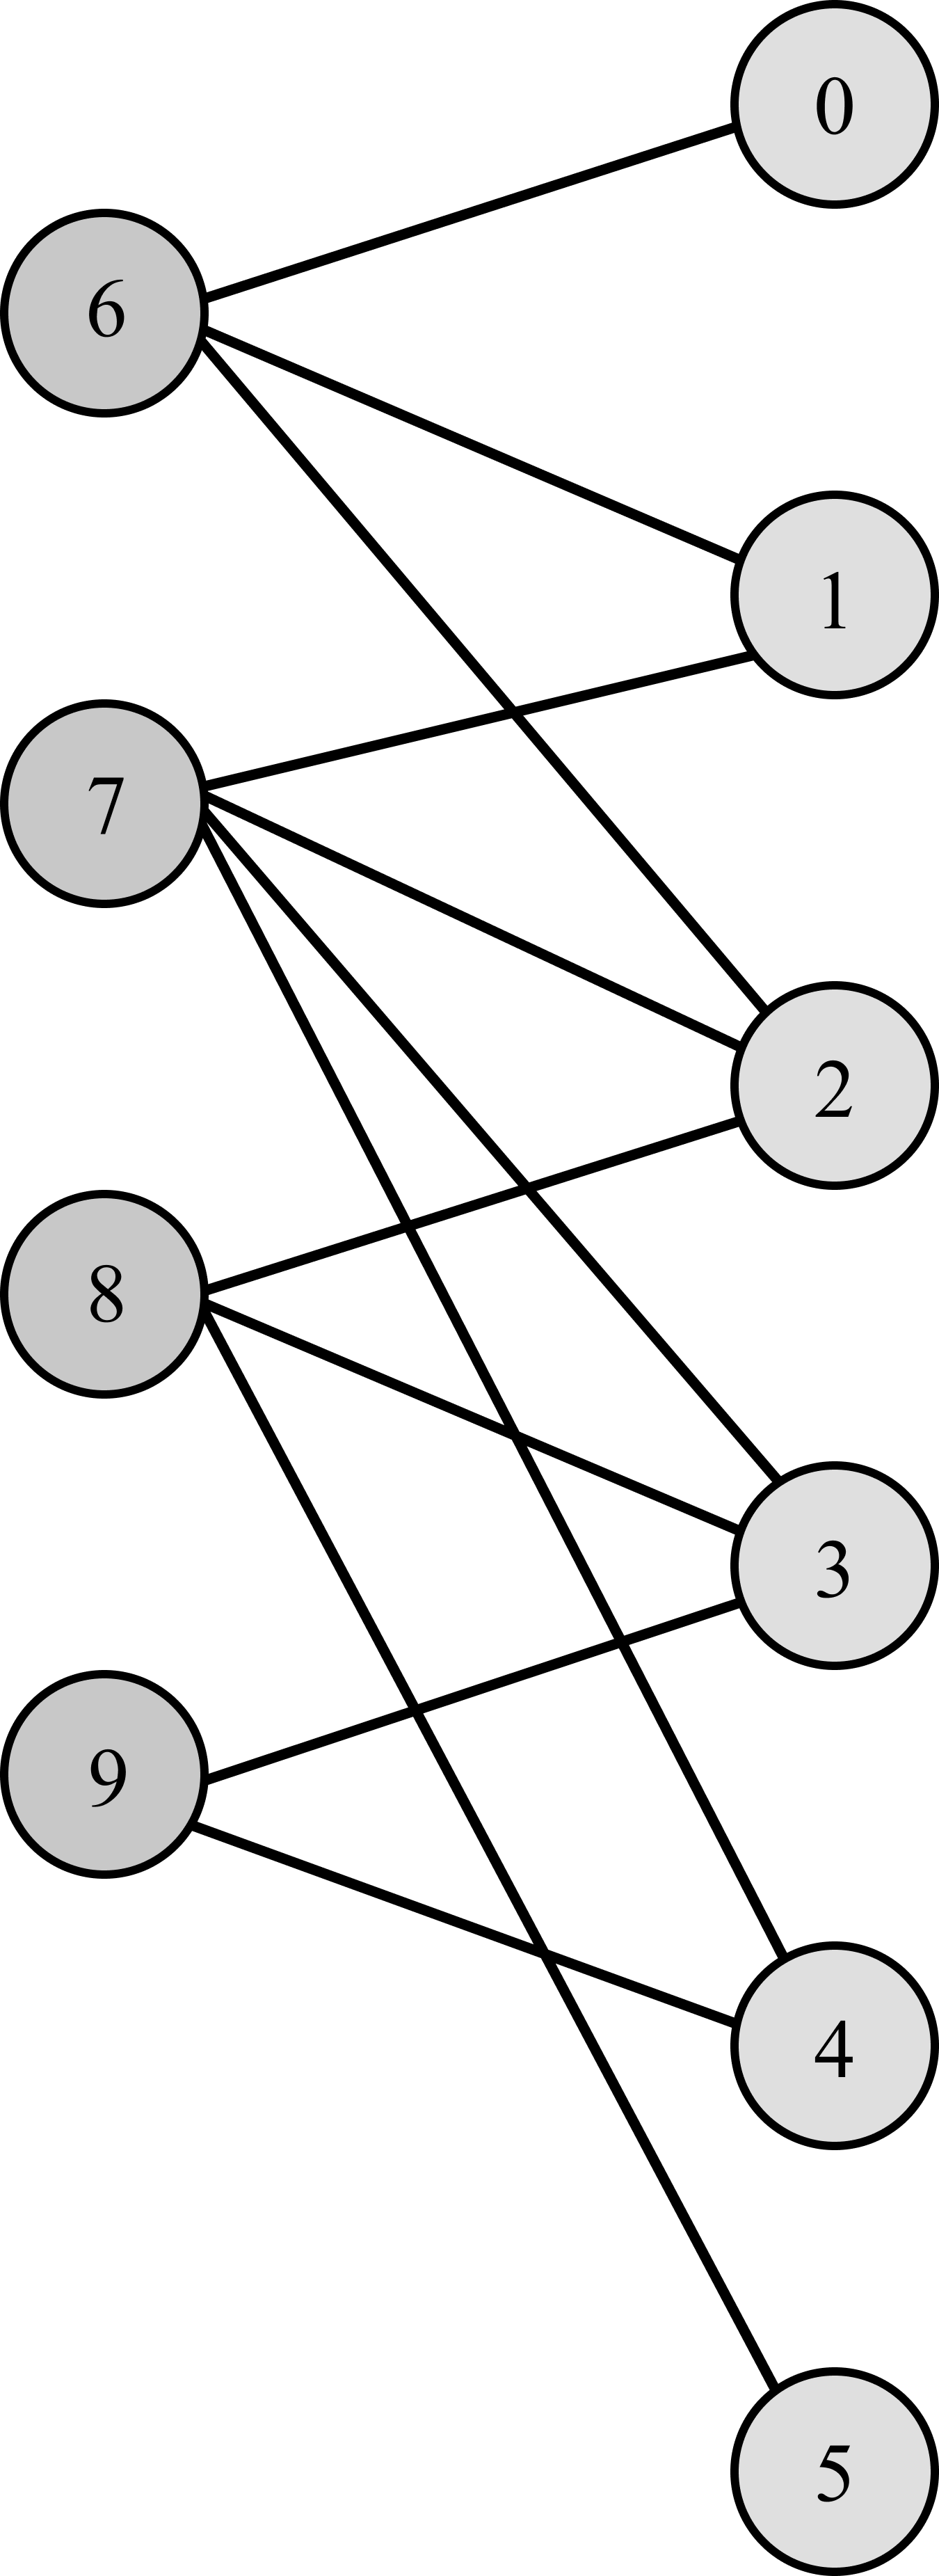
\includegraphics[height=7cm]{figures/bipartite.png} }}%
    \qquad
    \subfloat[\centering Example Peeling Space ]{{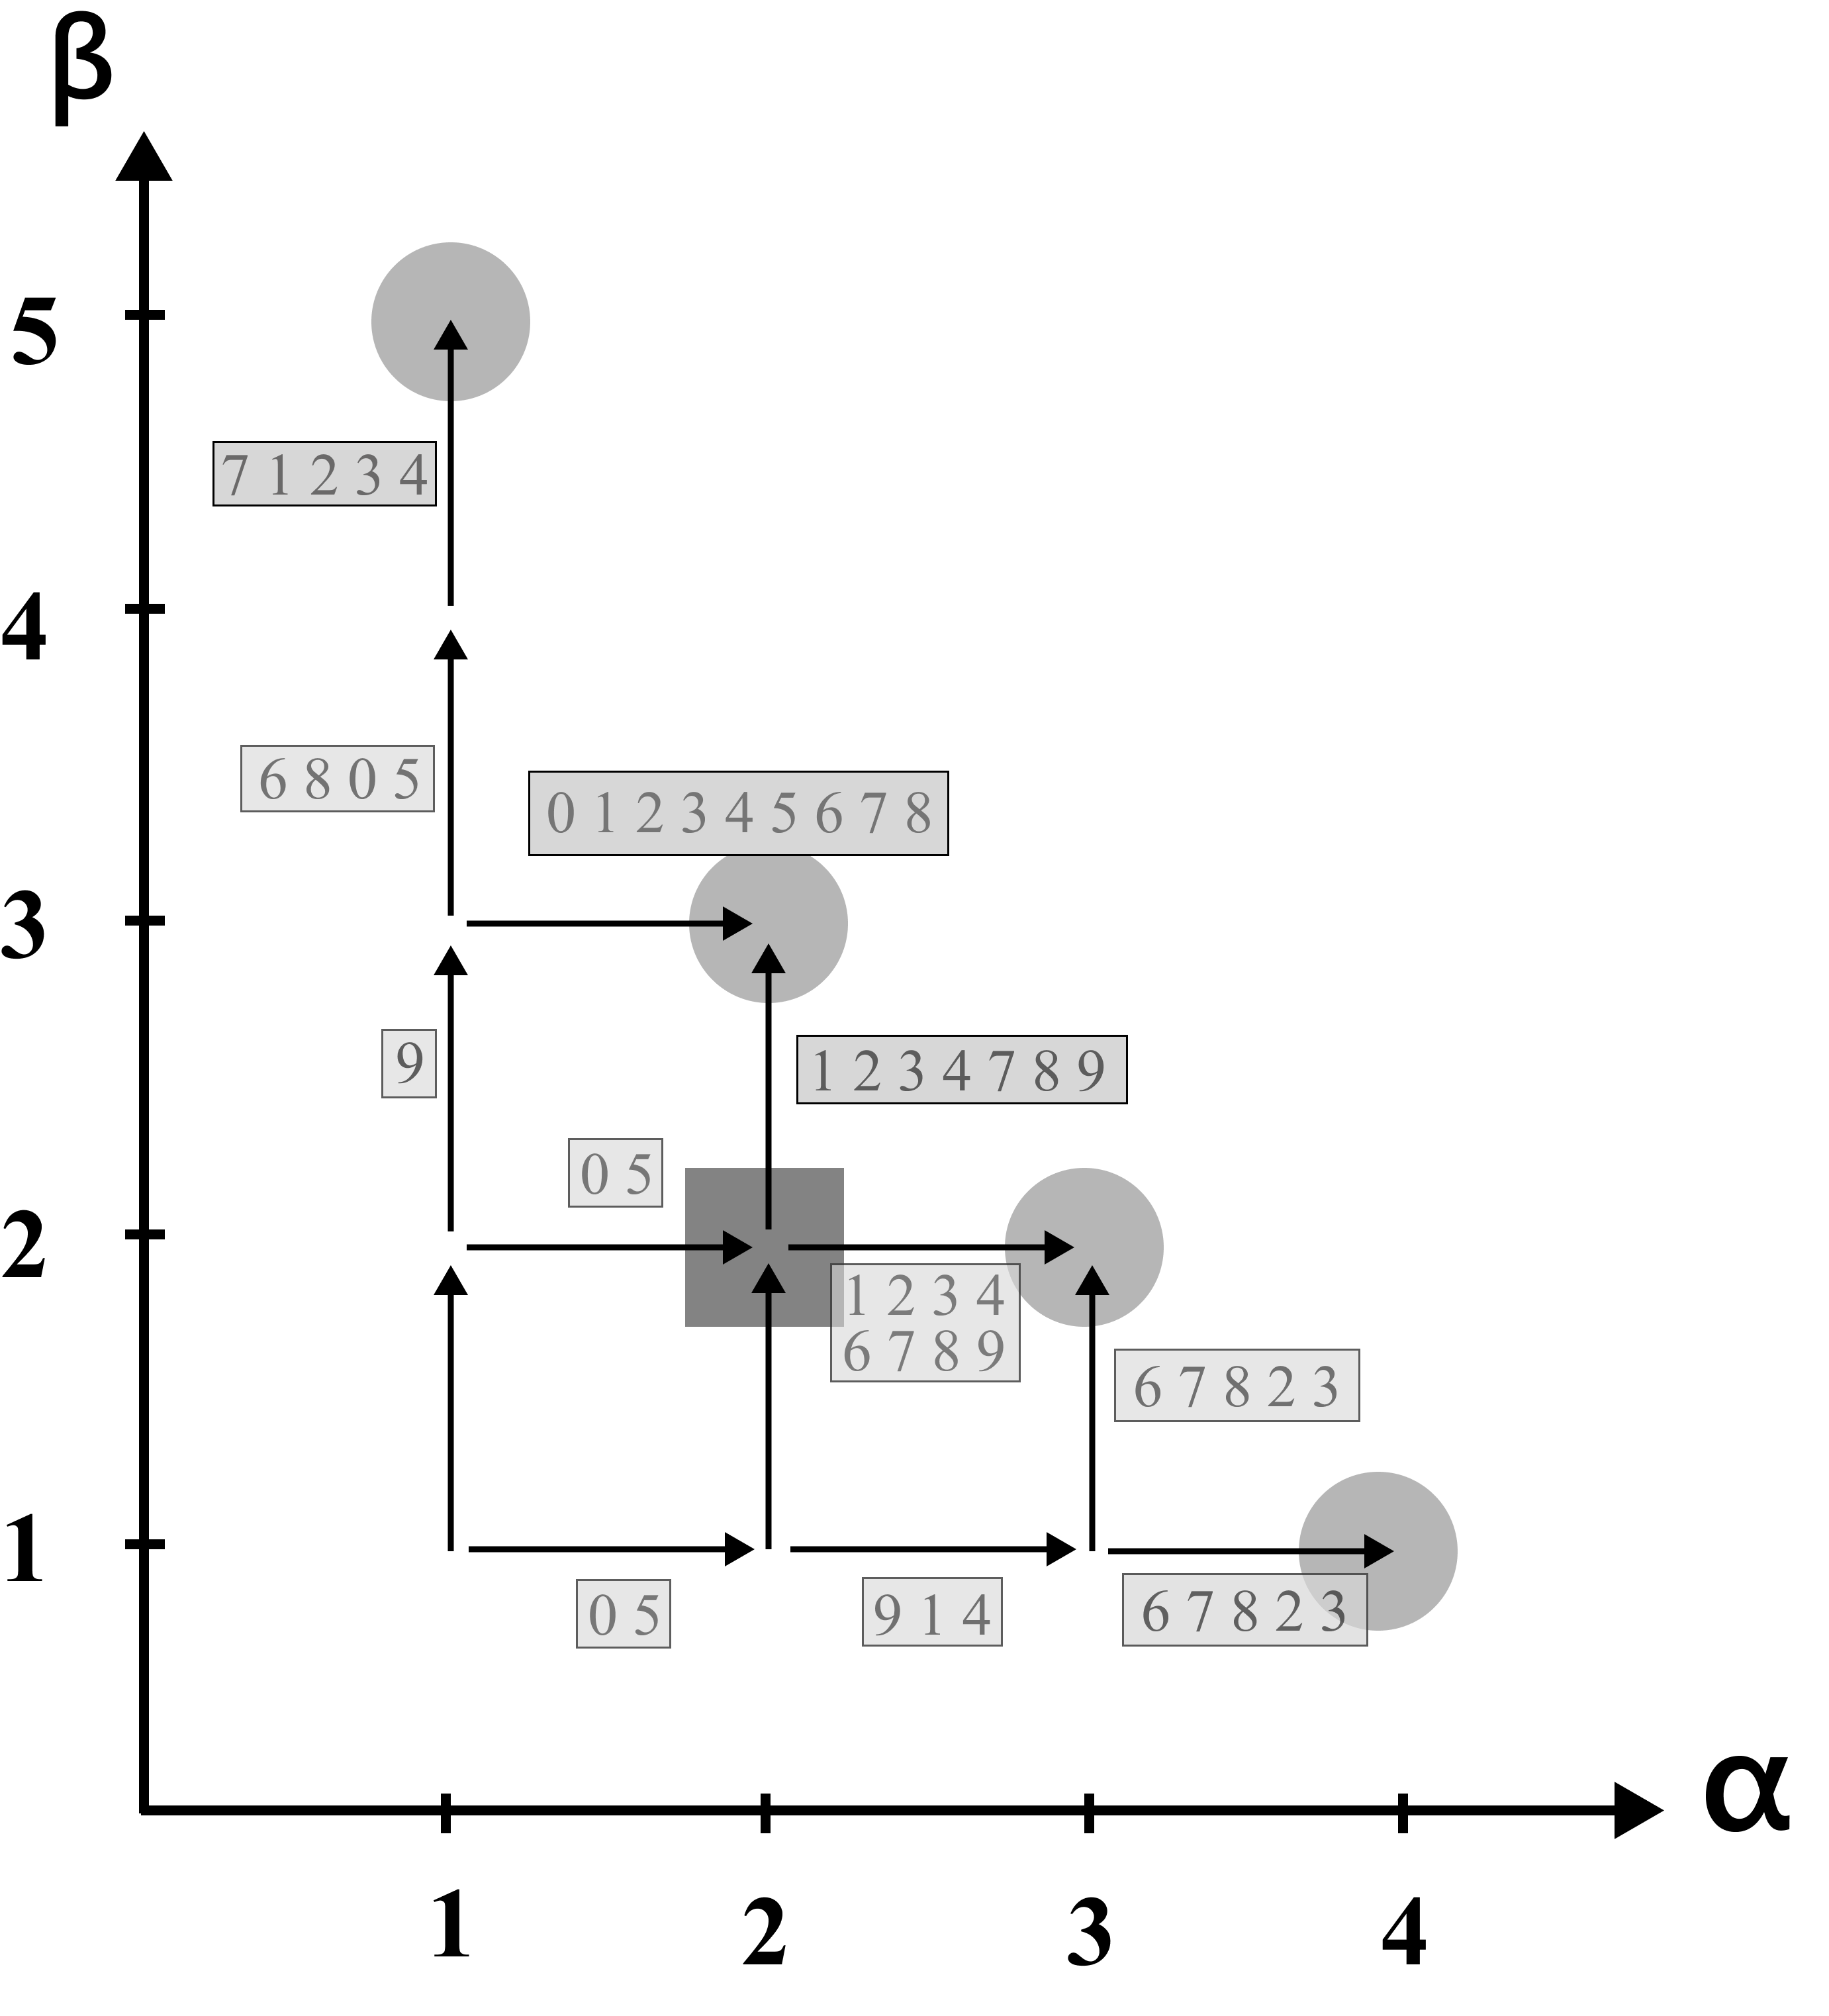
\includegraphics[width=7cm]{figures/diagram1.png} }}%
    \caption{On the left is an example bipartite graph, and on the right is an illustration of the peeling space of the graph. This is discussed in more detail in Section \ref{sec:optim}}%
    \label{fig:peel}%
\end{figure}

\begin{figure}%
    \centering
    \subfloat[\centering Algorithm \ref{alg-par}'s Peeling Path]{{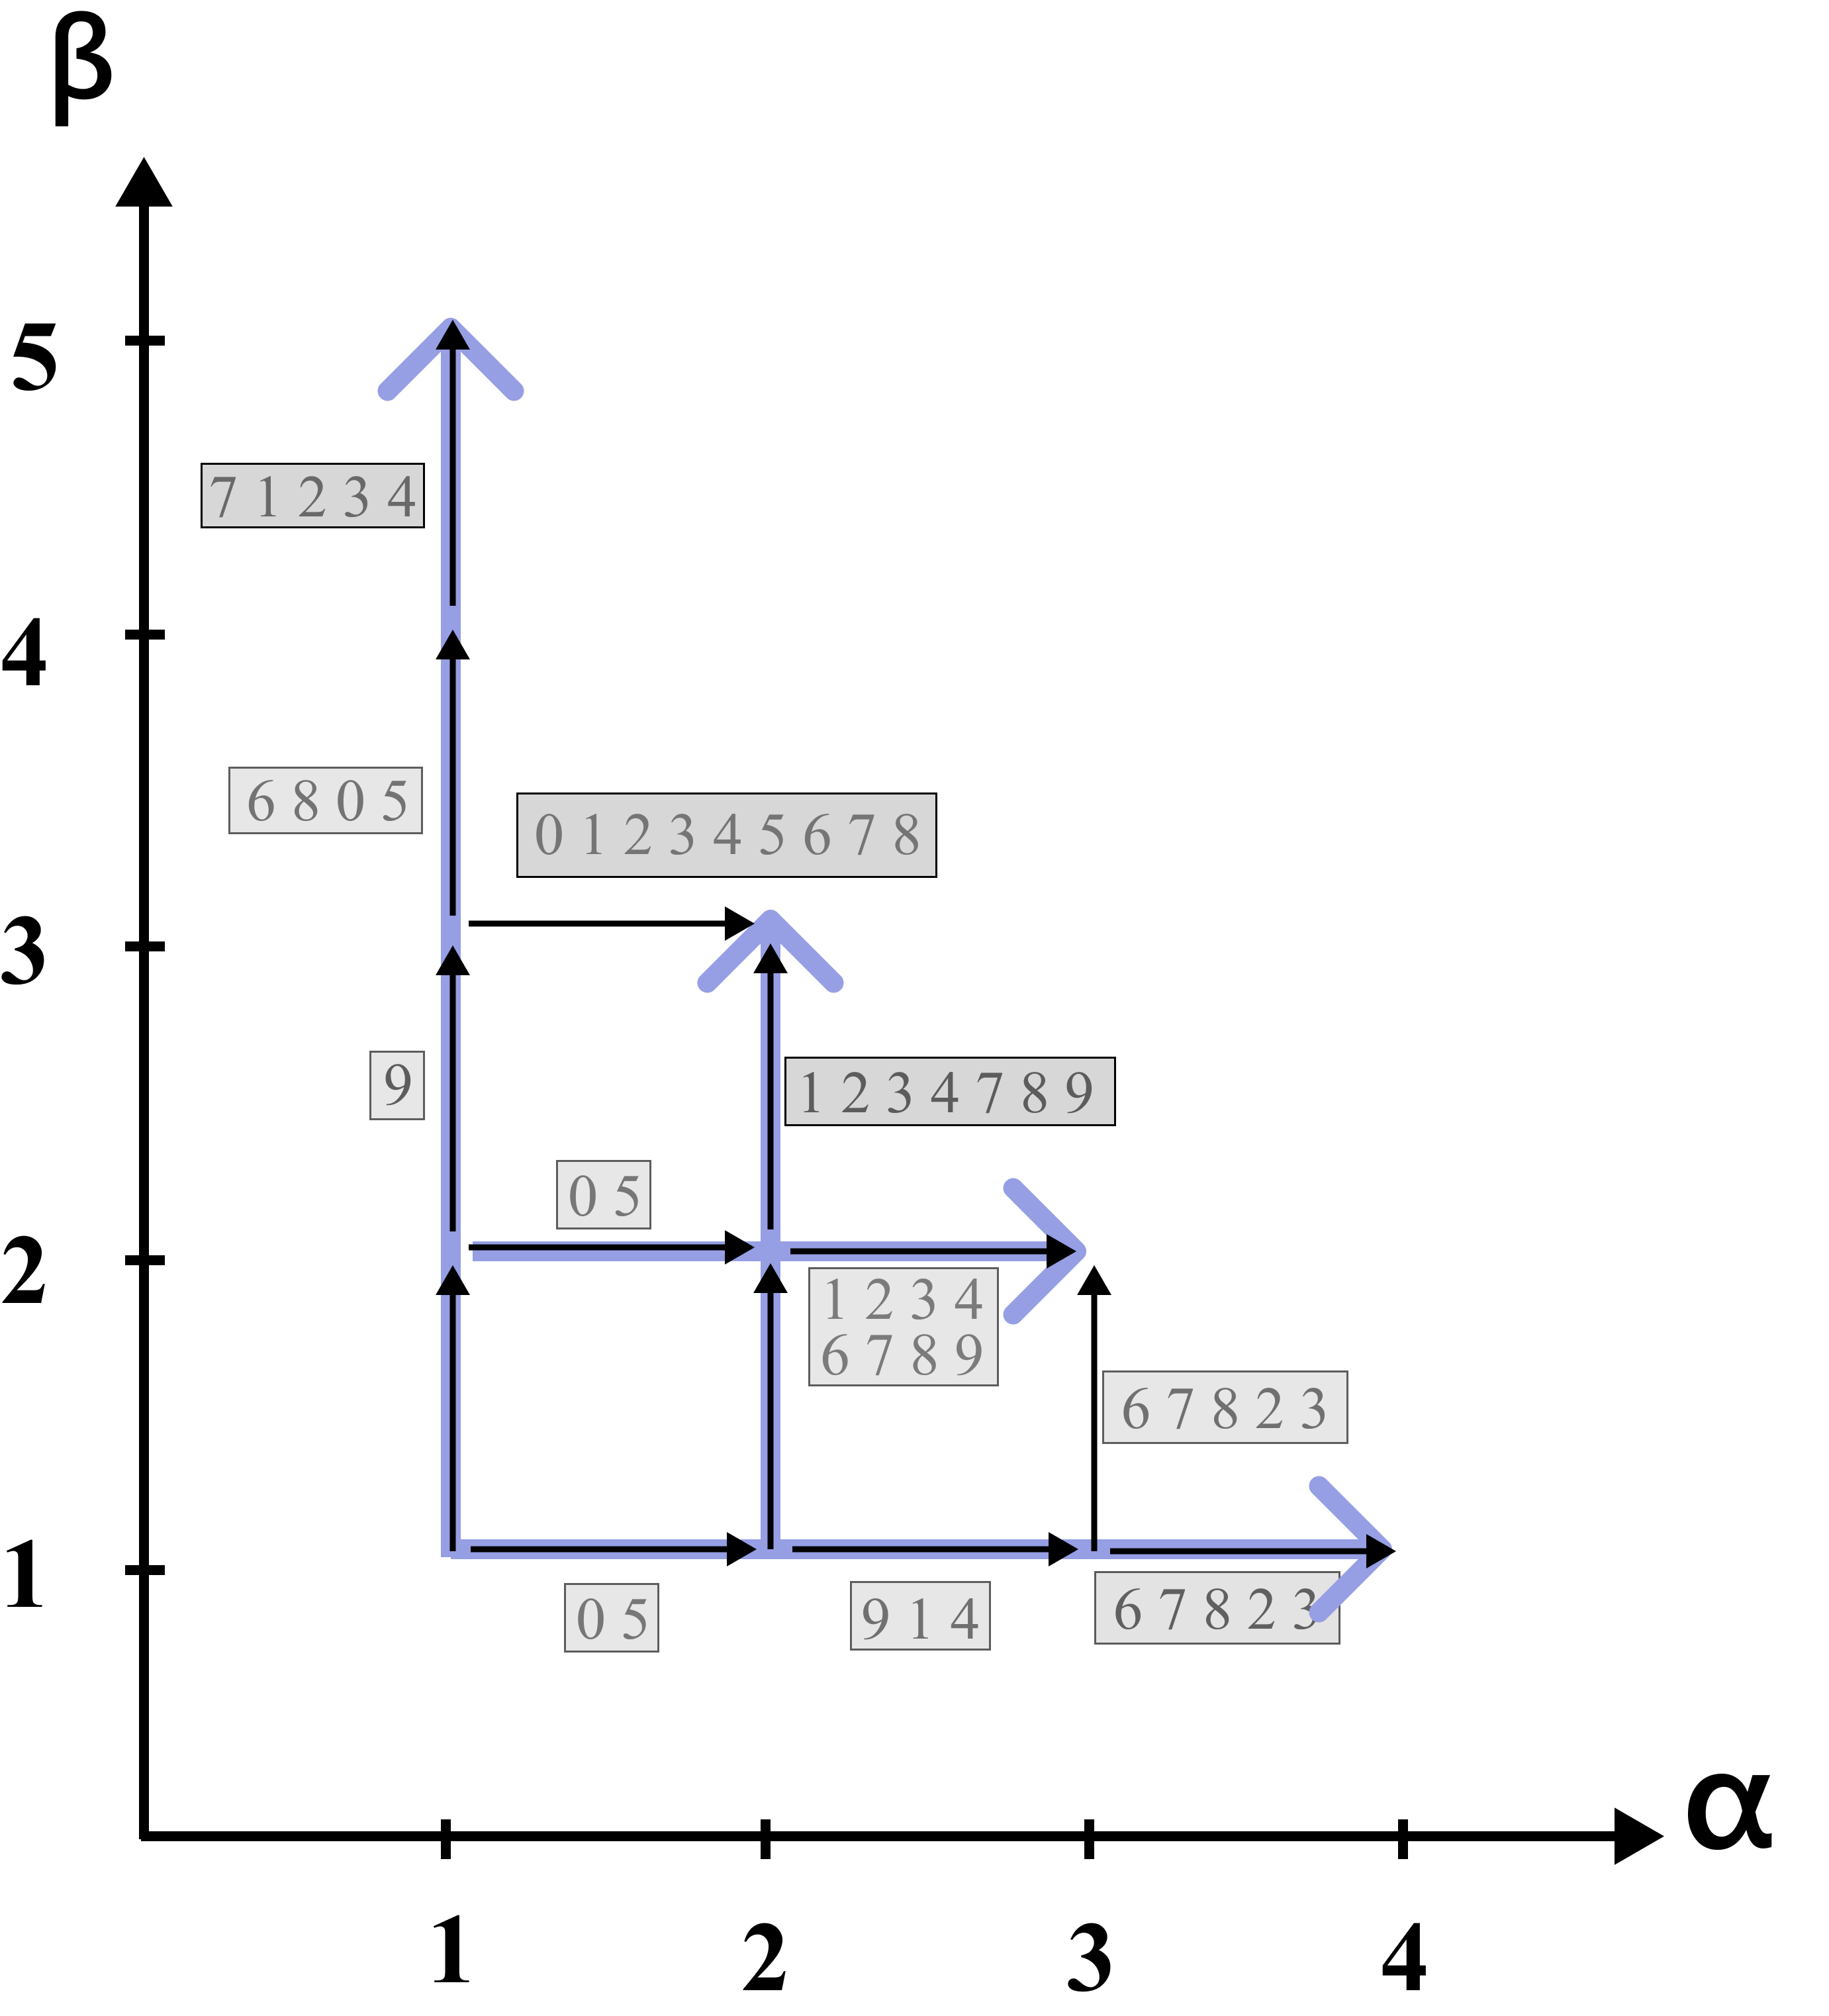
\includegraphics[width=7cm]{figures/diagram2.png} }}%
    \qquad
    \subfloat[\centering Optimized Peeling Path ]{{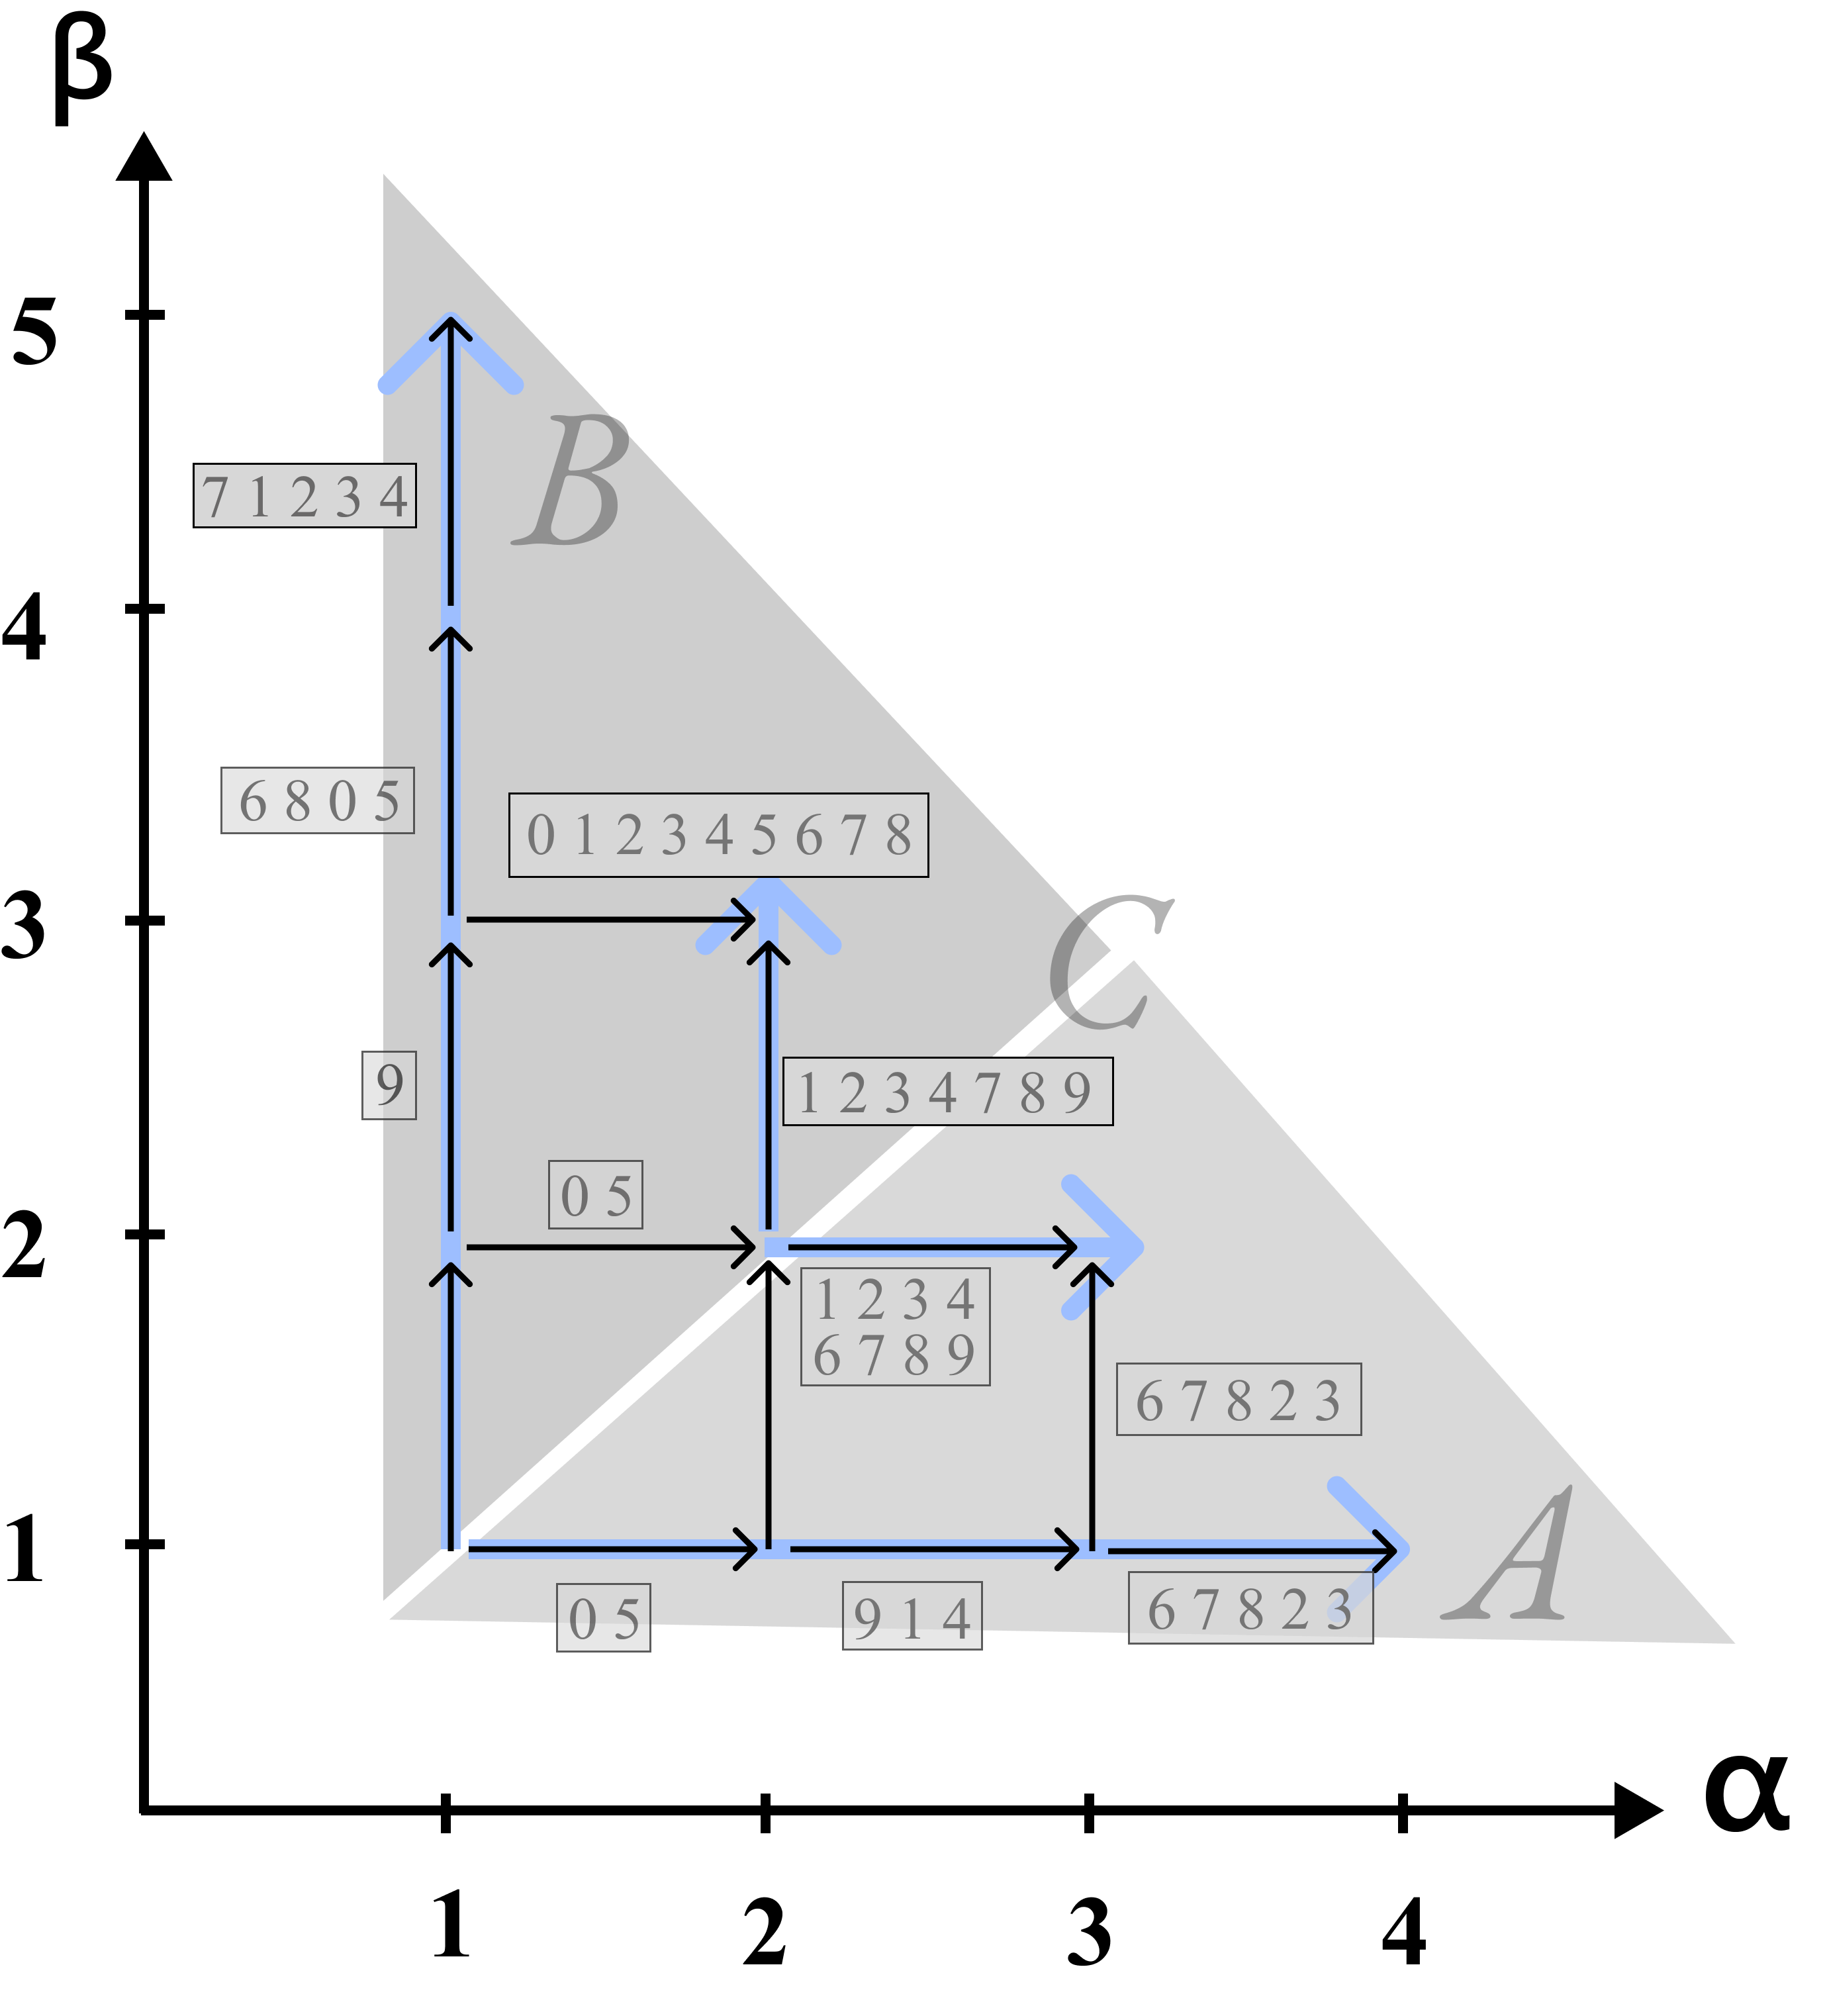
\includegraphics[width=7cm]{figures/diagram3.png} }}%
    \caption{This figure compares unoptimized vs optimized peeling paths. The left hand side shows the unoptimized peeling paths while the right hand side shows the optimized ones.}%
    \label{fig:peelspace}%
\end{figure}

Each integral intersection in the grid of Figure \ref{fig:peel} represents an $(\alpha,\beta)$-core. Edges represent a single-step peeling operation from $(\alpha,\beta)$-core to $(\alpha,\beta+1)$-core (upward) or to $(\alpha+1,\beta)$-core (rightward). The numerals on an edge represents the indices of vertices that would be deleted by that specific peeling operation. The circled nodes represent $(\alpha,\beta)$-cores that are empty, and the boxed node represents the $(\delta,\delta)$-core. Every core corresponding to a grid position that is not drawn is empty. The circled nodes form the boundary of the peeling space.

The peeling operations performed by Algorithm \ref{alg-par} can be visualized by the blue highlighted peeling paths in Figure \ref{fig:peelspace} (a). For $\alpha'=1$, we perform $\beta$-core peeling from $\beta=1$ to $\beta=5$. For $\alpha'=2$, we again increase $\beta$ from $1$ to $3$ while iteratively removing vertices not within the current bi-core. With the proposed optimization, for $\alpha'=2$, we only perform peeling from $\beta=2$ to $\beta=5$, starting from the $(\alpha',\alpha')$-core, or the $(2,2)$-core in this case. This is represented by the blue highlighted peeling paths in Figure \ref{fig:peelspace} (b).

To show the correctness of the optimized algorithm, we divide the peeling space into $3$ parts: part C with the diagonal $(x,x)$-cores, part B where all the $(\alpha,\beta)$-cores satisfy $\beta>\alpha$ and part A where the $(\alpha,\beta)$-cores satisfy $\alpha>\beta$. Note that part A of the peeling space corresponds visually to the part of peeling space below the diagonal $(x,x)$-cores; part B corresponds instead to the section above the diagonal $(x,x)$-cores. Thus, for the optimized algorithm, when peeling along increasing $\alpha$ values, it operates in part A of the peeling space; when peeling along increasing $\beta$ values it operates in part B of the peeling space. 

First, we note that the correct $\alpha_{\max \beta}(v)$ values are computed for all vertices $v$ with $(\alpha_{\max \beta}(v), \beta)$-cores in part A or C of the peeling space. For a specific $\beta$ value, if vertex $v\in (\alpha,\beta)$-core but $v\not\in (\alpha+1,\beta)$-core, with $\alpha\ge \beta$, then $\alpha_{\max \beta}(v)$ is recorded correctly to be $\alpha$ as we perform peeling along $\alpha$ values from $\alpha = \beta$ to its maximum value. 

Then, we show that the optimized algorithm computes the correct $\alpha_{\max \beta}(v)$ values for all vertices $v$ with $(\alpha_{\max \beta}(v), \beta)$-cores in part B of the peeling space. When peeling along increasing $\beta$ values with $\alpha' = \alpha_{\max \beta}(v)$, the algorithm would remove $v$ at $(\alpha_{\max \beta}(v), \beta')$-core, where $\beta'$ is some core value higher than $\beta$.
Given that, the updates of $\alpha_{\max \beta}(v)$ in \algname{par-peel-fix-$\alpha$} in Algorithm \ref{alg-par} as described in Section \ref{sec:par-decomp} ensures the $\alpha_{\max \beta}(v)$ value recorded is $\alpha'$, the correct value. Because A, B, and C form the entire peeling space, we have shown that for all $\beta$ and $v$ values, $\alpha_{\max\beta}(v)$ is correctly recorded. 

Symmetric correctness arguments can be established for $\beta_{\max \alpha}(u)$ values to show that the overall optimized algorithm is correct. 



\section{Parallel Bi-core Index Structure}\label{sec:parindex}

To allow for linear-time queries of $(\alpha,\beta)$-cores, we parallelize the indexing structure introduced by Liu \textit{et al.} \cite{Liu2020Efficient}. In this section, we discuss our parallel index construction and query algorithms. Both algorithms are work-efficient. The index construction algorithm has $\BigO{\log(n)}$ span, and the query algorithm has $\BigO{1}$ span.

We define $\mathbb{PI}^U, \mathbb{PI}^V$ to be the parallel index structures for the $U, V$ vertex partitions respectively. $\mathbb{PI}^U$ is the parallel version of $\mathbb{I}^U$, and $\mathbb{PI}^U_{\alpha, \beta}$ is the parallel version of $\mathbb{I}^U_{\alpha, \beta}$. Again, due to symmetry, we only discuss $\mathbb{PI}^U_{\alpha,\beta}$. $\mathbb{PI}^U_{\alpha,\beta}$ is a set containing the same elements as $\mathbb{I}^U_{\alpha,\beta}$ for any combination of $\alpha, \beta$. %The main structural difference lies in their implementation. 
In Liu \textit{et al.}'s work, each set $\mathbb{I}^U_{\alpha,\beta}$ is stored separately, pointed to within $\mathbb{I}^U$. In our parallelization, we store all the sets of vertices contiguously in an array, ordered first by their $\alpha$ value and then by their $\beta$ value. 
We call this array $\text{P}$. 
This is similar to the compressed sparse row (CSR) format used in graph representations. 
Then, we define $\text{M}$, a 2D jagged array where each $\text{M}[\alpha][\beta]$ corresponds to a set $\mathbb{PI}^U_{\alpha,\beta}$ and contains the starting index of that set in the array $\text{P}$. By definition, $\mathbb{PI}^U_{\alpha,\beta}=$ all vertices in $\text{P}$ in range $\left[\text{M}[\alpha][\beta], \text{M}[\alpha][\beta+1]\right)$. 

This way, $\left[\text{M}[\alpha][\beta], \text{M}[\alpha+1][0]\right)$ directly gives the range of vertices in $\text{P}$ that corresponds to $\bigcup_{i = \beta}^{\max_\beta(\alpha)} \mathbb{PI}^U_{\alpha,i} = (\alpha,\beta)$-core.

Thus, to query the $(\alpha,\beta)$-core, we return all vertices in $P$ in the range $\left[\text{M}[\alpha][\beta],\text{M}[\alpha+1][0]\right)$. This takes $\BigO{|(\alpha,\beta)\text{-core}|}$ work and $\BigO{1}$ span.


\subsection{Parallel Index Construction}

% \jessica{Introduce pseudocode first -- "The pseudocode for our parallel index construction algorithm is in Algorithm ...". (I guess you do this later, but in that case, you shouldn't mention Algorithm x here. Just say the objective of our parallel index construction algorithm is...}
The objective of the index construction algorithm is to take as input $\beta_{\max \alpha}(u)$ for every $u\in U$ and construct M and P. 

To construct P, we perform parallel \algname{radix-sort} on the vertices based on their $\alpha,\beta$ values. Then, we use a parallel filter to find the indices at which the $\alpha \text{ or } \beta$ value differs, which we store in an array $\text{TPT}$ (total pointer table). We also find indices where the $\alpha$ value differs, which we store in $\text{FPT}$ (first pointer table). Then, using these two pointer tables, the 2D jagged array $\text{M}$ is constructed. 
% mention CSR

\begin{algorithm}
 \footnotesize
\caption{Parallel Index Construction}
 \begin{algorithmic}[1]
 
 \Procedure{Build-U-Index}{$\beta_{\max}$} 
 \State $\text{P}\leftarrow$ list of $(\alpha, \beta_{\max \alpha}(u), u)$ for every $u\in U$ \label{par-index:list}
 \State \algname{radix-sort}($\text{P}$) \Comment{Sorts the list of tuples by first $\alpha$, then $\beta$ values} \label{par-index:radix}
 \State Initialize $\text{TPT}$ \Comment{Creates an empty $\text{TPT}$ with the same size as $\text{P}$}
 \ParFor{$i=0$ to $\text{P}.\text{size}-1$}
    \If{$i=0$ or $\text{P}$[$i-1$].$\alpha \not =$ $\text{P}$[$i$].$\alpha$ or $\text{P}$[$i-1$].$\beta \not = \text{P}$[$i$].$\beta$}
        \State $\text{TPT}$[$i$]$\leftarrow i$ \Comment{Records index location where $\alpha$ or $\beta$ changes value}
    \EndIf
 \EndParFor
 \State \Call{filter}{$\text{TPT}$, element is not empty} \Comment{Filter out empty indices in $\text{TPT}$}
 \State Initialize $\text{FPT}$ \Comment{Creates an empty $\text{FPT}$ with the same size as $\text{TPT}$}
 \ParFor{$i=0$ to $\text{TPT}.\text{size}-1$}
    \If{$i=0$ or $\text{P}$[$\text{TPT}$[$i-1$]].$\alpha \not =$ $\text{P}$[$\text{TPT}$[$i$]].$\alpha$}
        \State $\text{FPT}$[$i$]$\leftarrow i$ \Comment{Records index location on $\text{TPT}$ array of where $\alpha$ value changes}
    \EndIf
 \EndParFor
 \State \Call{filter}{$\text{FPT}$, element is not empty} \Comment{Filter out empty indices in $\text{FPT}$}
 \State Initialize $\text{M}$ \Comment{Creates empty $\text{M}$ array with $1\text{st}$ dimension $= \text{FPT}.\text{size}$ and $2^\text{nd}$ dimension $= \max_\beta(\alpha)$}
 \ParFor{$\alpha=1$ to $\text{FPT}.\text{size}$}
    \ParFor{$j=\text{FPT}$[$\alpha-1$] to $\text{FPT}$[$\alpha$]$-1$}
        \State $\text{start}\leftarrow \text{TPT}$[$j$] \Comment{Gets start index location of $j^\text{th}$ block}
        \State $\text{M}$[$\alpha$][$\text{P}$[$\text{start}$].$\beta$] $\leftarrow\text{start}$ \Comment{Stores start location; $\text{P}[\text{start}].\beta$ gives $j^\text{th}$ block's corresponding $\beta$ value}
    \EndParFor
    \State $\text{M}$[$\alpha$] $\leftarrow$ \algname{suffix-min}($\text{M}$[$\alpha$])
 \EndParFor
 \State \Return $\text{M}$ 
 \EndProcedure
 
 \Procedure{Build-V-Index}{$\alpha_{\max}$} 
 \State symmetric to \algname{build-u-index}
 \EndProcedure
 \end{algorithmic}
 \label{alg-ind-cons}
\end{algorithm}

The pseudocode for our parallel index construction algorithm is given in Algorithm \ref{alg-ind-cons}. We now discuss our algorithm in more detail.
First, on Line \ref{par-index:list}, we store a list of tuples $(\alpha, \beta_{\max \alpha}(u), u)$ to $\text{P}$. This is the list of all possible combinations of $\alpha$ and vertex $u\in U$, with the $\beta_{\max \alpha}(u)$ value attached. We perform parallel \algname{radix-sort} on $\text{P}$ based on the ordering of first the $\alpha$ values and then the $\beta$ values on Line \ref{par-index:radix}. We initialize an empty $\text{TPT}$ on Line 4 with the same size as $\text{P}$. The parallel for loop on Lines 5--8 finds all indices at which either the $\alpha$ value or the $\beta$ value in $\text{P}$ changes. 
This is accomplished by marking the indices where changes happen on Line 7 and filtering out all the unmarked index positions on Line 8. Constructing $\text{TPT}$ essentially breaks up the array $\text{P}$ into blocks where each block has constant $\alpha,\beta$ value and corresponds to set $\mathbb{PI}^U_{\alpha, \beta}$. $\text{TPT}[i]$ records the starting index location of the $i^\text{th}$ block. Lines 9--13 repeats the entire process, but for $\text{FPT}$ to filter out index positions where the $\alpha$ value of $\text{P}$ changes. Note that the indices stored in $\text{FPT}$ are not indices of positions in $\text{P}$. Instead, they are indices of positions in $\text{TPT}$. $\left[\text{FPT}[\alpha-1],\text{FPT}[\alpha]\right)$ gives the range of blocks defined by $\text{TPT}$ that has this particular $\alpha$ value. It corresponds to set $\mathbb{PI}^U_{\alpha}$. 

Finally, based on $\text{FPT}$ and $\text{TPT}$, we create $\text{M}$ in the following manner. We obtain $\text{M}[\alpha]$ for each $\alpha$ value independently. Line 16 iterates in parallel over the blocks that have the particular $\alpha$ value. For each block $j$, we store its starting position $\text{TPT}[j]$ to $\text{M}[\alpha][\beta_j]$ where $\beta_j$ is the $\beta$ value corresponding with the $j^\text{th}$ block. This is done on lines 17--18. Now, we have constructed $\text{M}[\alpha][\beta']$ correctly for all $(\alpha,\beta')$ pairs such that $\beta'$ appears in $\beta_{\max \alpha}(u)$ for some $u\in U$. 

For pairs $(\alpha, \beta)$ such that $\beta$ does not appear in $\beta_{\max \alpha}(u)$ for some $u\in U$, we point $\text{M}[\alpha][\beta]$ to the same destination as $\text{M}[\alpha][\beta']$ where $\beta'$ is the smallest value larger than $\beta$ and appears in $\beta_{\max \alpha}(u)$ for some $u\in U$. We accomplish this by performing \algname{suffix-min} on $\text{M}[\alpha]$ on Line 19.


\myparagraph{Analysis}
Since $\text{P}.\text{size} = \BigO{m}$, the work is bounded by $\BigO{m}$ since all operations on lines 3--14 have linear work with respect to the length of the array input. Lines 15--19 have work complexity $\BigO{m}$, because we loop through the $\text{M}$ table exactly once and from Section \ref{sec:seqindex}, we know the table takes $\BigO{m}$ space.

Algorithm \ref{alg-ind-cons} has span $\BigO{\log(n)}$ \textit{w.h.p.}, since \algname{radix-sort}, \algname{filter}, and all other operations are bounded by $\BigO{\log(m)} = \BigO{\log(n)}$ span \textit{w.h.p.}. 


% \subsection{Parallel Bi-core Query}

% \begin{algorithm}
%  \footnotesize
% \caption{Parallel Bi-core Query}
%  \begin{algorithmic}[1]
 
%  \Procedure{Query-U}{$\alpha$, $\beta$} 
%     \If{$\alpha$, $\beta$ does not exist in $\text{M}$}
%         \State \Return $\emptyset$
%     \EndIf
%     \State $\text{start}\leftarrow \text{M}$[$\alpha$][$\beta$] 
%     \State $\text{end}\leftarrow \text{M}$[$\alpha+1$][$0$] 
%     \State \Return \algname{slice}$(\text{P},\text{start}, \text{end})$ \Comment{Slice the array $\text{P}$ from start to end (exclusive) in parallel}
%  \EndProcedure
%  \end{algorithmic}
%  \label{alg-ind-q}
% \end{algorithm}

%parallelization explanation
\section{Experiments}

% mention practical implementation (use intro to provide a roadmap)

In this section, we provide a comprehensive evaluation of our implementations of parallel bi-core algorithms.

\subsection{Experiment Setup}

We use real-world graphs from the KONECT graph database \cite{Kunegis13}, the details of which are given in Table \ref{tab:graphs}. Specifically, we used the graphs, in descending number of edges, Orkut, Web Trackers, LiveJournal, Delicious, TREC, Reuters, Epinions, Flickr.
%The graphs we used (shown in Table \ref{tab:graphs}) are Orkut~\cite{konect:2017:orkut-groupmemberships}, Web Trackers~\cite{konect:2017:web-trackers}, LiveJournal~\cite{konect:2017:livejournal}, epinions~\cite{konect:2017:epinions}, TREC~\cite{konect:2017:gottron-trec}, flickr~\cite{konect:2017:flickrEdges}, and reuters~\cite{konect:2017:reuters}.

We use Google Cloud Platform \texttt{c2-standard-60} instances for all our experiments, which are 30-core machines with two-way hyper-threading, with Intel 3.1 GHz Cascade Lake processors and 240 GB of memory; the processors have a max turbo clock-speed of 3.8 GHz.

% should probably box it like an actual paper
\begin{table*}[t]
 \begin{tabular}{|| c c c c c c c c c ||} 
 \hline
 Graph Name & Type & $|U|$ & $|V|$ & $n$ & $m$ & $\text{dmax}$ & $\delta$ & $\rho_{\text{max}}$ \\ [0.5ex] 
 \hline
 Orkut & Membership & 2.78M & 8.73M & 11.51M & 327M & 318K & 466 & 12100 \\
 \hline
 Web Trackers & Inclusion & 27.7M & 12.7M & 40.43M & 140.6M & 11.57M & 437 & 4542 \\
 \hline  
 LiveJournal & Membership & 3.20M & 7.49M & 10.69M & 112M & 1.05M & 108 & 6831 \\
 \hline
 Delicious & Purchase & 833K & 33.7M & 34.6M & 101.8M & 143K & 183 & 4771 \\
 \hline
 TREC & Inclusion & 556K & 1.17M & 1.73M & 83.6M & 457K & 508 & 6029 \\
 \hline
 Reuters & Inclusion & 781K & 284K & 1.06M & 60.6M & 345K & 192 & 4767 \\
 \hline
 Epinions & Rating & 120K & 755K & 880k & 13.67M & 162K & 151 & 3049 \\
 \hline
 Flickr & Membership & 396K & 104K & 500k & 8.55M & 35K & 147 & 2300 \\
 \hline
\end{tabular}
\caption{\label{tab:graphs}Data and information on tested graphs.}
\end{table*}


\subsection{Implementation and Other Optimizations}

While our parallel bi-core decomposition algorithm, given in Algorithm \ref{alg-par}, is theoretically efficient, it is practically slow due to the overhead incurred by the histogram-based \algname{par-del-update} subroutine. We find that its high parallelism fails to compensate for this overhead.

To implement a practically fast bi-core decomposition algorithm, we do not implement the fully parallelized version of our algorithm, and only parallelize between different calls of \algname{par-peel-fix-$\alpha$} and \algname{par-peel-fix-$\beta$}. This practical parallel algorithm, which corresponds to \algname{par-baseline}, is similar to the parallel algorithm introduced by Liu \textit{et al.} \cite{Liu2020Efficient}; however, our implementation differs from theirs in that we employ a lazily instantiated bucketing structure, where we only instantiate a constant number of buckets at any given time in our bucketing structure. 
This technique was introduced by Dhulipala \textit{et al.}~\cite{DhBlSh17} for implementing their $k$-core decomposition algorithm. We further apply the peeling space pruning optimization to \algname{par-baseline} to obtain \algname{par-optimized}.

To reiterate, the $6$ algorithms we implement are 

\begin{enumerate}
    \item \algname{seq-baseline}: Algorithm \ref{alg-seq}, the state of the art sequential algorithm proposed by Liu \textit{et al.}
    \item \algname{seq-optimized}: Algorithm \ref{alg-seq}, but with peeling space pruning optimization introduced in section \ref{sec:optim}
    \item \algname{par-baseline}: Liu \textit{et al.}'s parallel algorithm, but with an optimized bucketing structure
    \item \algname{par-optimized}: \algname{par-baseline}, but with the peeling space pruning optimization
    \item \algname{par-index}: Algorithm \ref{alg-ind-cons}
    \item \algname{par-query}: Parallel index query algorithm described in Section \ref{sec:parindex}.
\end{enumerate}

We use the Graph Based Benchmark Suite~\cite{dhulipala20} to implement our algorithms. All code is written in C++ with the -O$3$ optimization level enabled. We perform each experiment 3 times and report the average running time.

Despite the difference in machines, with Liu \textit{et al.} reporting their runtimes on a 3.4 GHz CPU, our sequential baseline closely reproduces the result reported by Liu \textit{et al.}~\cite{Liu2020Efficient}. The paper reported a runtime of 4103 seconds for their sequential algorithm, while our reproduction attains a runtime of 4539 seconds. We are not able to obtain their source code. 


\subsection{Bi-core Decomposition}

In this section, we report the runtime of the $4$ bi-core decomposition algorithms \algname{seq-baseline}, \algname{seq-optimized}, \algname{par-baseline}, and \algname{par-optimized}. 

\begin{figure}%
    \centering
    \subfloat[\centering runtimes (log-scale)]{{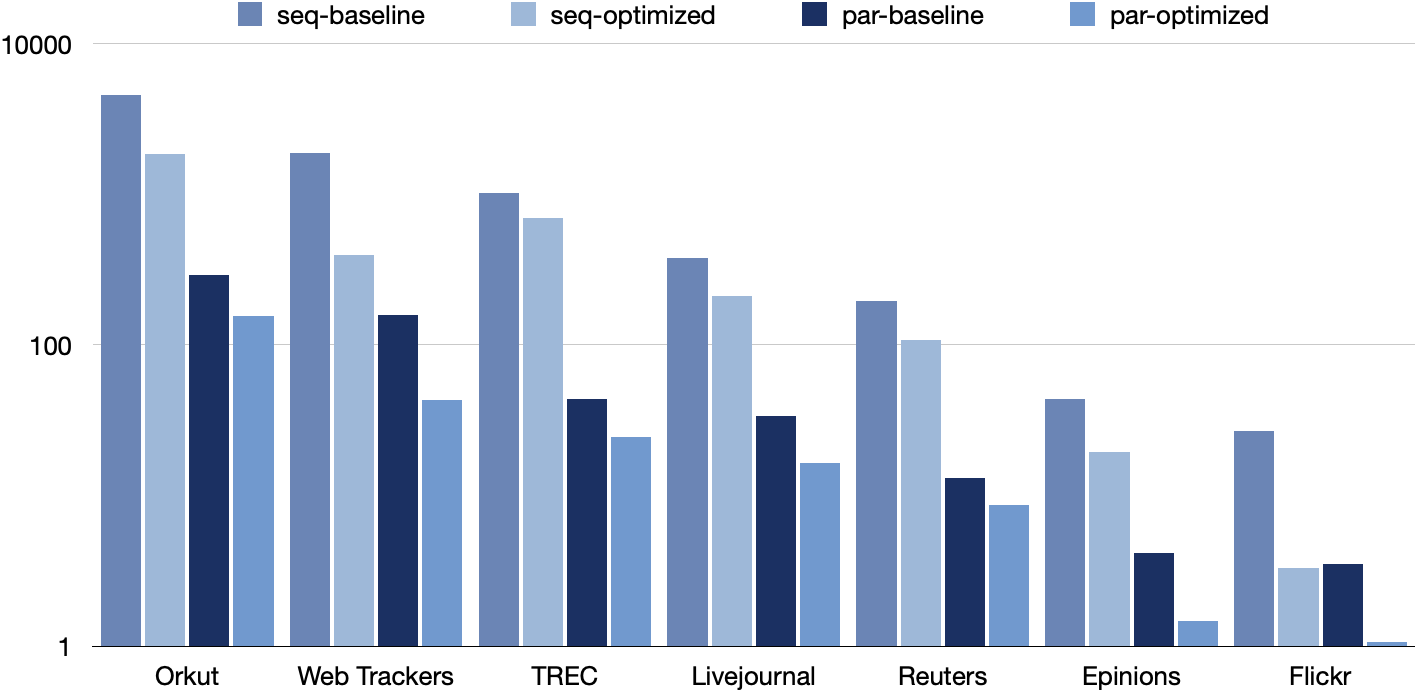
\includegraphics[width=7cm]{figures/log-runtime-comp.png} }}%
    \qquad
    \subfloat[\centering runtimes ]{{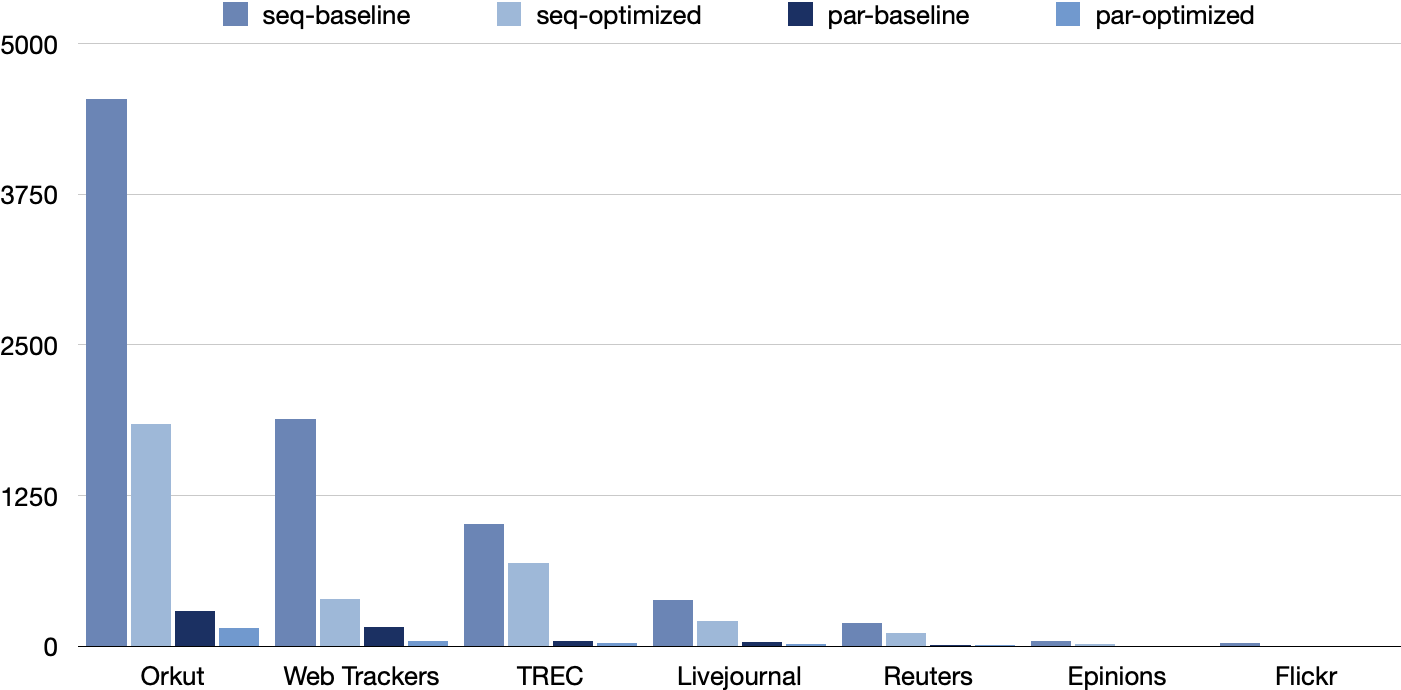
\includegraphics[width=7cm]{figures/linear-runtime-comp.png} }}%
    \caption{This figure comparatively shows the runtime (in seconds) of the 4 bi-core decomposition algorithms, \algname{seq-baseline}, \algname{seq-optimized}, \algname{par-baseline}, \algname{par-optimized}. Graph (a) is in log-scale while graph (b) is in linear-scale. \algname{par-optimized} consistently performs all 3 other algorithms.}%
    \label{fig:runtimes}%
\end{figure}

\myparagraph{Performances Comparison}

Figure \ref{fig:runtimes} shows the runtimes of the $4$ algorithms for graphs in Table \ref{tab:graphs}. The parallel algorithms are run with 30 threads. We do not run on 60 threads because the extra threads are hyperthreads and are not actual cores. Therefore, we observed that using 60 hyperthreads did not improve our running times.

\algname{par-baseline} and \algname{par-optimized} significantly outperforms \algname{seq-baseline} and \algname{seq-optimized}. While the parallel algorithms can process graphs with hundreds of millions of edges within several minutes, the sequential algorithms can take more than an hour to finish.

Running on 30 threads, \algname{par-optimized} attains 23--44x speedup over \algname{seq-baseline}, the sequential state of the art.

To compare against the parallel state of the art, also introduced by Liu \textit{et al.}, we note that they reported a runtime for 12 threads of 732 seconds for the Orkut graph. On the other hand, still running on 12 threads, \algname{par-optimized} attains a runtime of 253 seconds for the Orkut graph. Thus, our algorithm achieves a 2.9x speedup over Liu \textit{et al.}'s parallel algorithm, demonstrating the effectiveness of out introduced optimizations.

% \jessica{Generally when comparing to other people's work, it's better to be a bit delicate about it and give them as much benefit of doubt as possible. In 7.2, when discussing other implementations, I'd put in this kind of comment where we were not able to obtain their source code (this is nicer than saying that we weren't able to compile their source code), which is why we implement our own baselines to compare against. Then, in 7.2, you'd also say something like, we compare against their reported numbers in our analysis. I would not mention the kind of CPUs their using -- just say that they get x time on x cores, and for the same number of cores, we obtain x time. Also, don't mention that they only report concrete numbers for orkut; just write the comparison for orkut, and leave it at that.}

Figure \ref{fig:runtimes} also demonstrates the effectiveness of the peeling space pruning optimization we introduce. \algname{seq-optimized} consistently outperforms \algname{seq-baseline} by 2.1-2.8x. Similarly, \algname{par-optimized} is about 1.6-4.2x faster than \algname{par-baseline}. This demonstrates the effectiveness of the optimization technique across sequential and parallel setting. 

\begin{figure}%
    \centering
    \subfloat[\centering Speedup Ratios for Tested Graphs]{{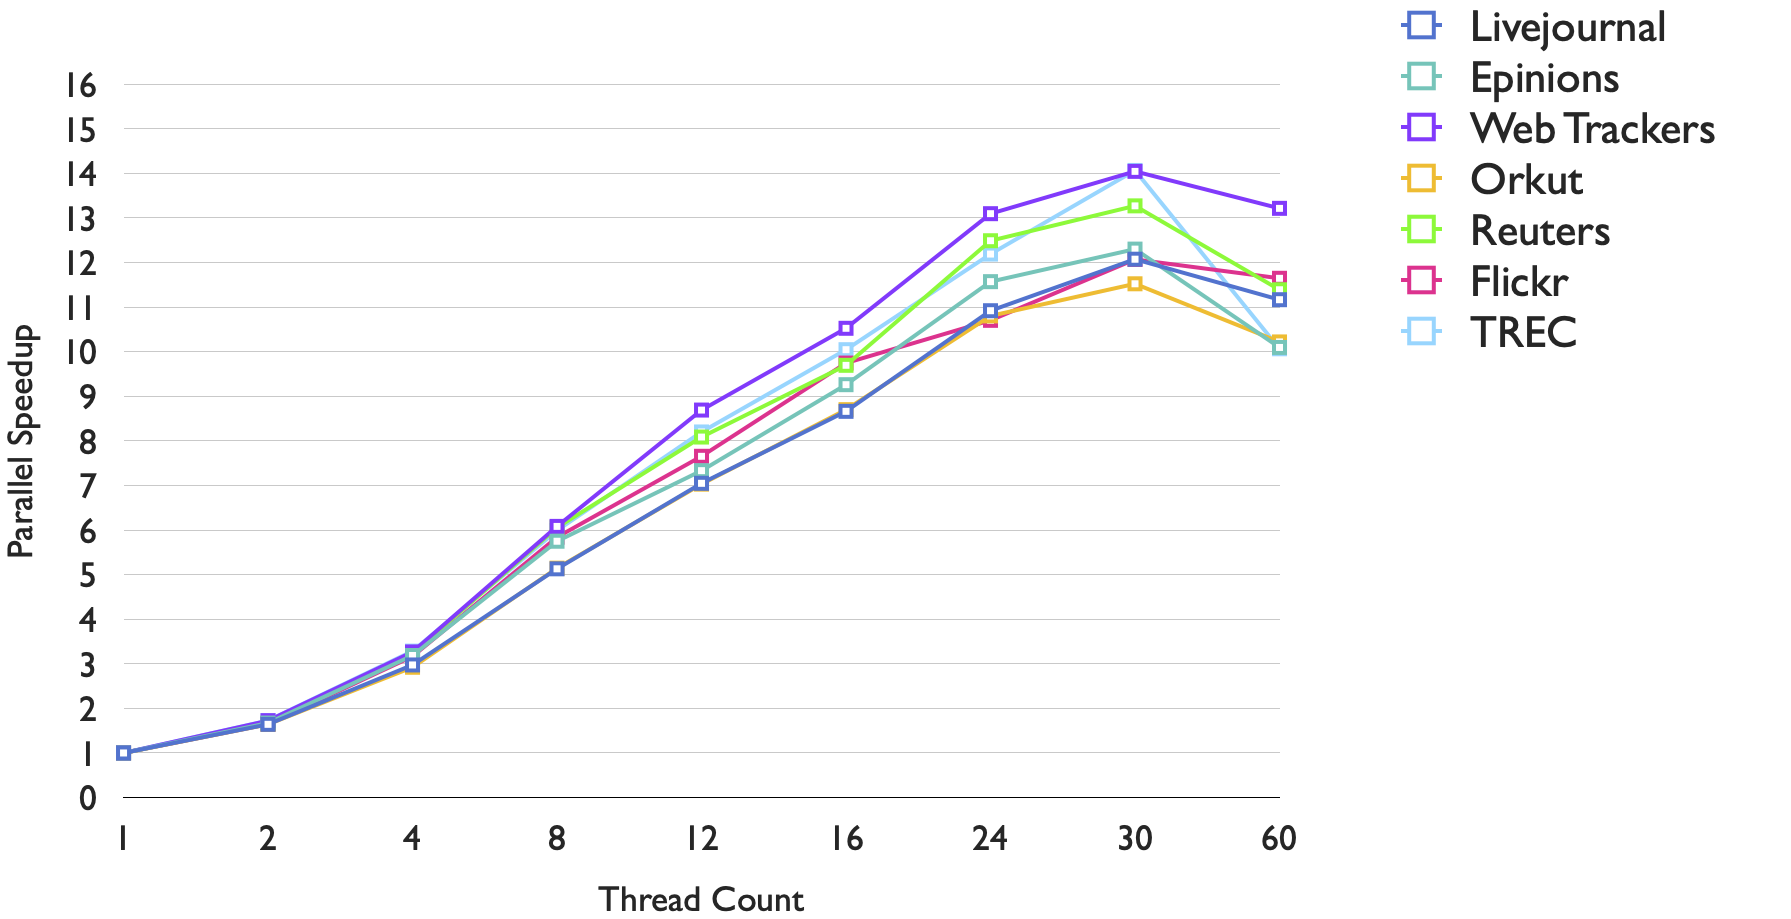
\includegraphics[width=7cm]{figures/speedup.png} }}%
    \qquad
    \subfloat[\centering Ratio of Runtimes Relative to Serial Time]{{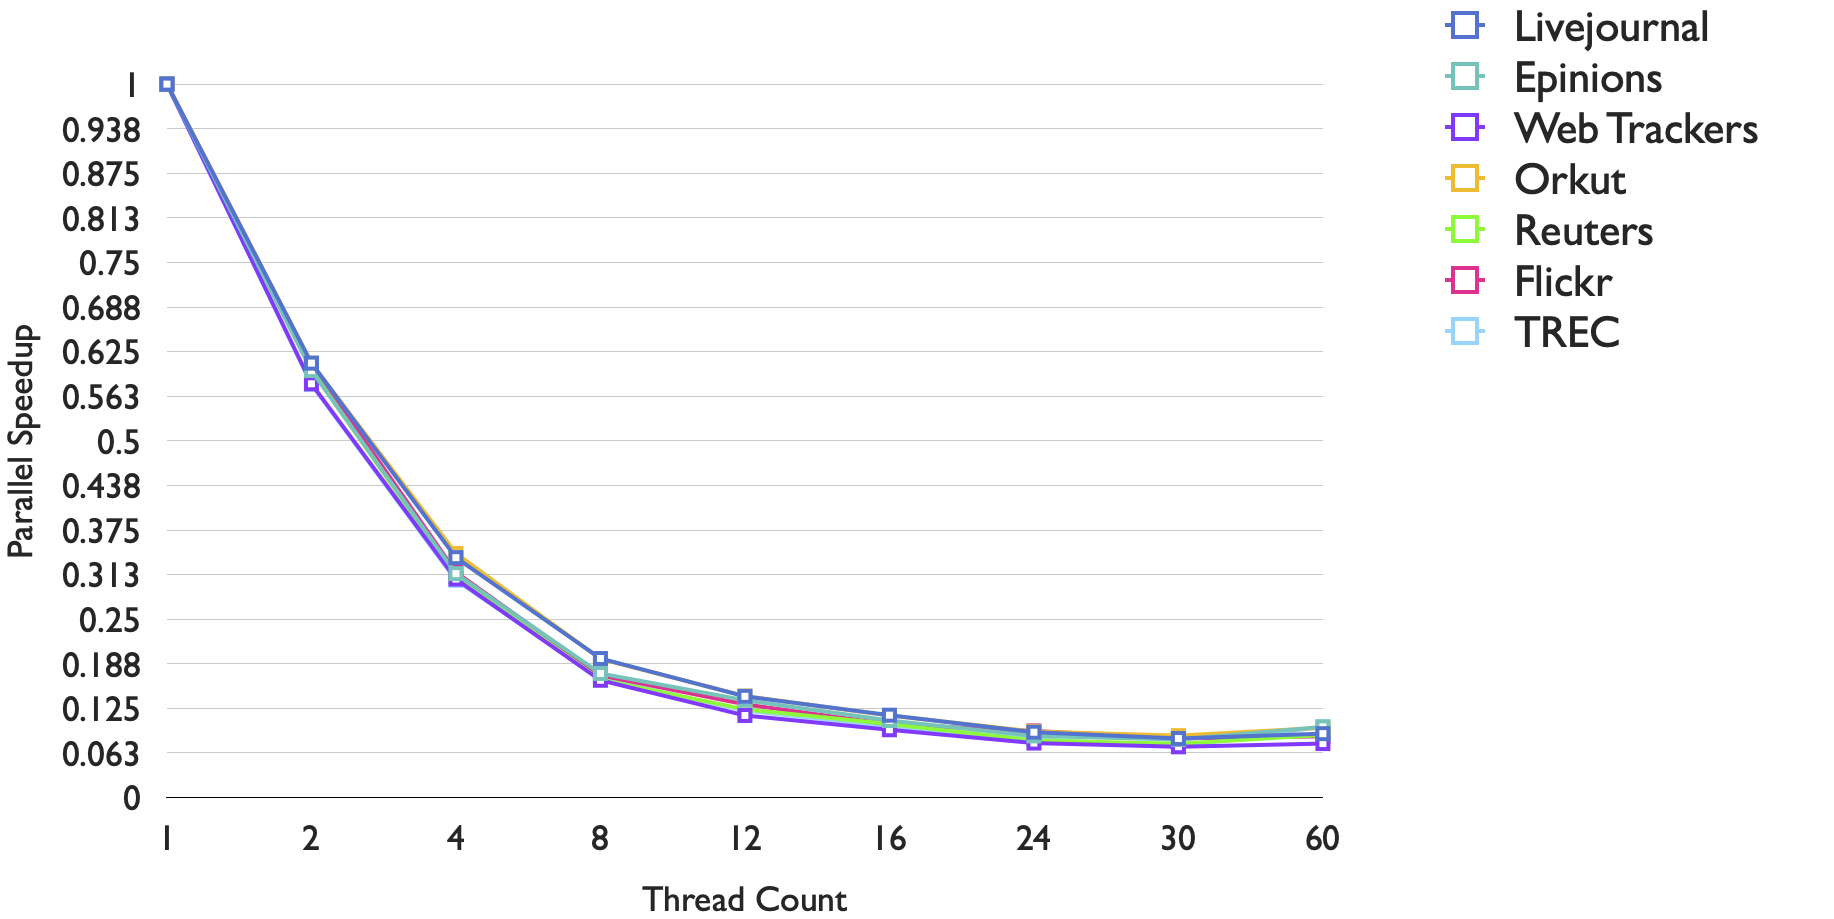
\includegraphics[width=7cm]{figures/runtime-ratio.png} }}%
    \caption{Graph (a) shows plots of the runtime of \algname{par-optimized} across different number of threads for various graphs. The plots show consistent speedups. Graph (b) shows the runtime ratios, which are the multiplicative inverses of the speedup numbers}%
    \label{fig:speedup}%
\end{figure}

\myparagraph{Analysis of Scalability}

As shown in Figure \ref{fig:speedup}, \algname{par-optimized} achieves a 11.5–14.1x self-relative speedup when running on 30 threads compared to 1 thread. The speedup plateaus at 60 threads. Increasing from 30 threads to 60 threads introduces virtual hyper-threads and not physical cores. So it is expected that there is no significant runtime improvement.

Further, Figure \ref{fig:speedup} demonstrates that the speedup achieved by \algname{par-optimized} is consistent across different graphs, showing that \algname{par-optimized} is scalable to graphs of sizes up to hundreds of millions of edges without noticeable deterioration in its parallel speedup. 

%\myparagraph{Analysis of $\rho$ vs runtime}

%\begin{figure}  
%\begin{center}  
%\includegraphics[width=0.8\columnwidth]{figures/rho-runtim%e.png}\caption{Rho value vs. Runtimes}\label{fig:rho}
%\end{center}  
%\end{figure}  

%The span of our algorithm is $\BigO{\rho \log(n)}$ \textit{w.h.p.} Theoretically, $\rho$ is bounded by $\BigO{\max(\text{dmax}_u,\text{dmax}_v)}=\BigO{n}$. Therefore, it is theoretically reasonable to assume that $\rho$ is the dominant term in the span. That is empirically true. For graphs given in Table \ref{tab:graphs}, the $\rho$ values are significantly larger than $\log_2(n)$ values. Thus, it is natural to assume there is an approximately linear correlation between the runtimes of \algname{par-optimized} and the $\rho$ values. Indeed, figure \ref{fig:rho} experimentally demonstrates a near-linear correlation between the $\rho$ values and the runtimes. This demonstrates that the bi-core peeling complexity we introduced is an important value in both theoretical and empirical evaluation of parallel bi-core decomposition algorithms.  

\subsection{Bi-core Index Construction}\label{sec:exp-index-cons}

\begin{figure}%
    \centering
    \subfloat[\centering Speedup Ratios for Tested Graphs]{{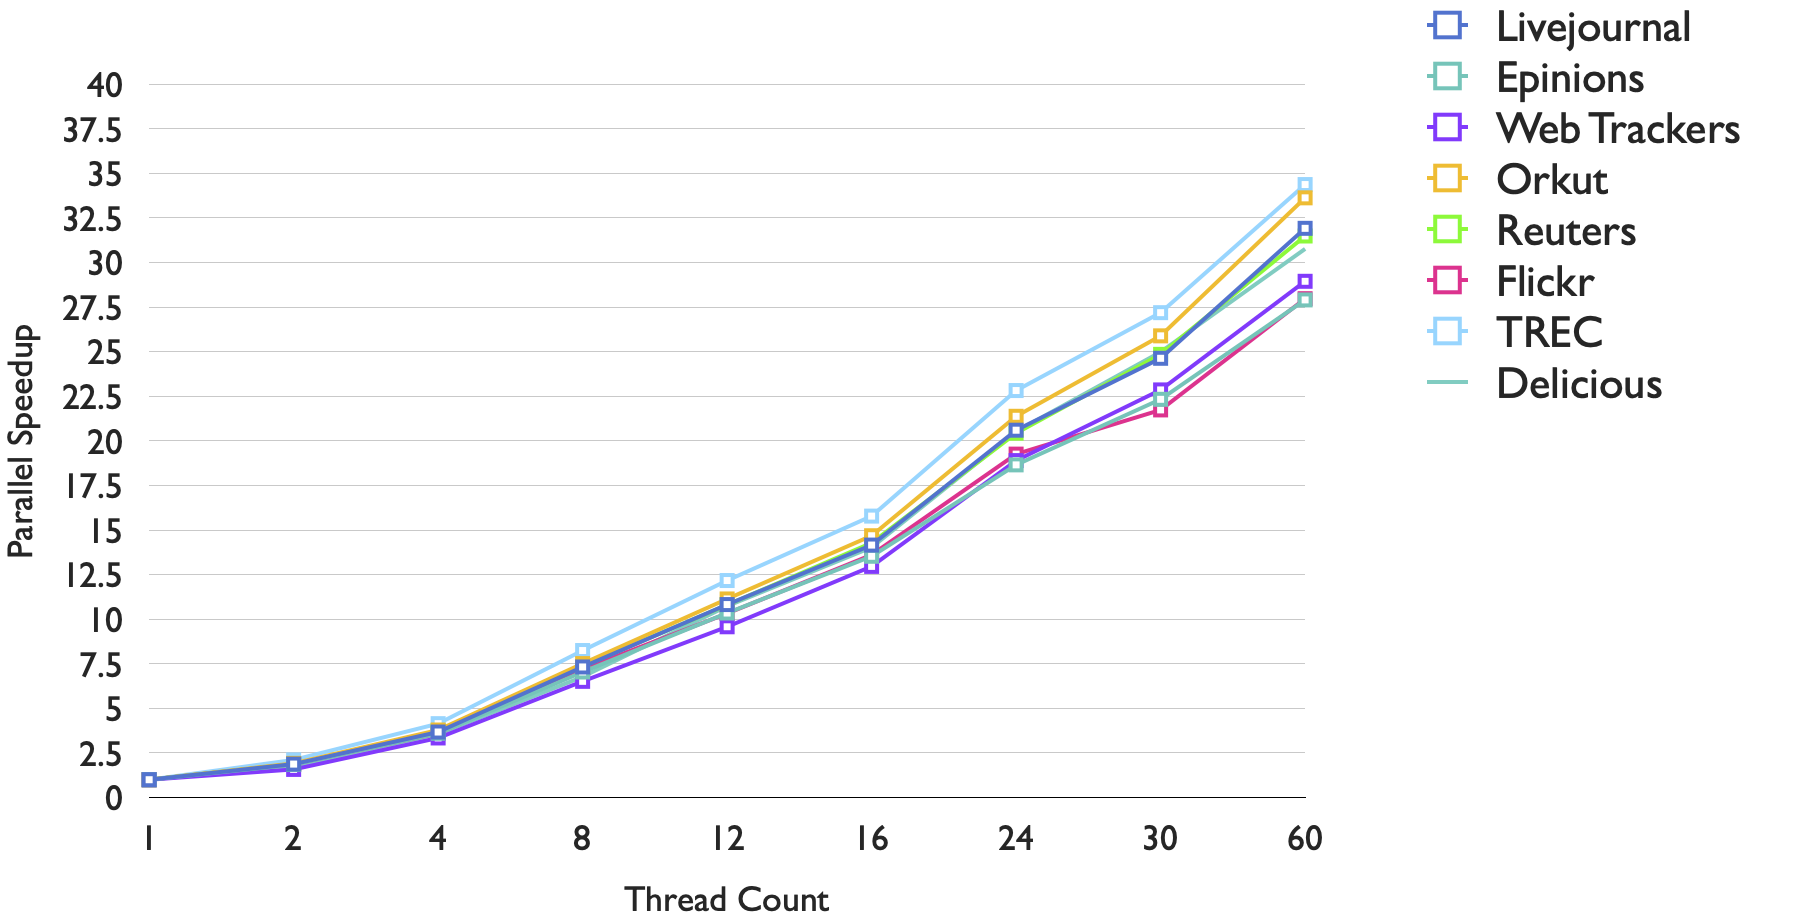
\includegraphics[width=7cm]{figures/speedup-cons.png} }}%
    \qquad
    \subfloat[\centering Ratio of runtimes relative to serial time]{{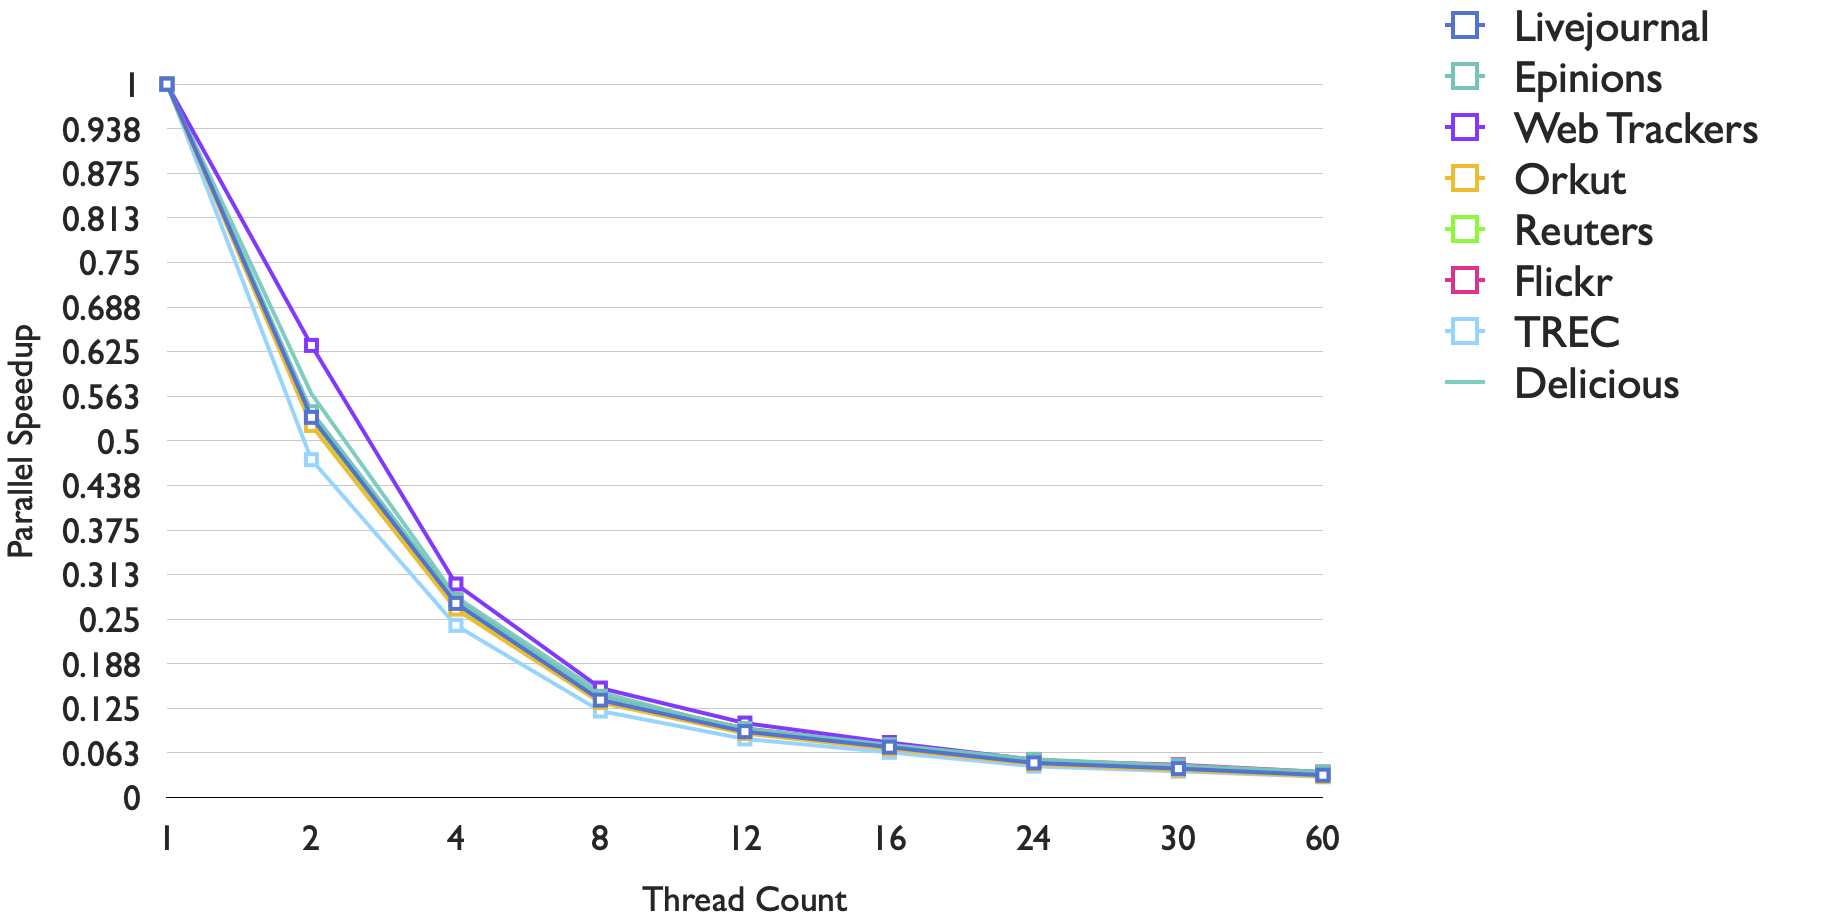
\includegraphics[width=7cm]{figures/runtime-ratio-cons.png} }}%
    \caption{Graph (a) shows plots of \algname{par-index}'s speedup over different number of threads used. Graph (b) shows the runtime ratios.}%
    \label{fig:speedup:c}%
\end{figure}

Now, we report the runtimes of the bi-core index construction algorithm, or \algname{par-index}. Using 30 threads, \algname{par-index} terminates for most graphs within several seconds. For example, when run on Orkut, a graph with 327 millions edges, with 30 threads, \algname{par-index} takes only 3.76 seconds to finish. This is $2.4\%$ of the runtime of \algname{par-optimized}. \algname{par-index} takes up similar percentage of time for other large graphs while taking up larger portion of time for smaller graphs. For example, on Flickr, \algname{par-index} is $10\%$ of \algname{par-optimized} in terms of runtime. This observation matches the theoretical prediction based on \algname{par-index}'s lower work complexity as compared to \algname{par-optimized}, which predicts that the runtime of \algname{par-optimized} grows faster than that of  \algname{par-index} as the number of edges increases.

\myparagraph{Analysis of Scalability}

Given its span of $\BigO{\log(n)}$, \algname{par-index} predictably has significant parallelism. Figure \ref{fig:speedup:c} demonstrates the parallel speedup of \algname{par-index} across different number of threads and different graphs used. Running on Delicious with 30 threads, \algname{par-index} achieves a near-linear self-relative speedup of 25.0x. A similar speedup number is achieved for all other graphs, as shown in Figure \ref{fig:speedup:c}. This demonstrates \algname{par-index} to be scalable to graphs of large sizes.

\subsection{Bi-core Index Query}\label{sec:exp-index-q}

\begin{figure}%
    \centering
    \subfloat[\centering Speedup ratios for tested graphs]{{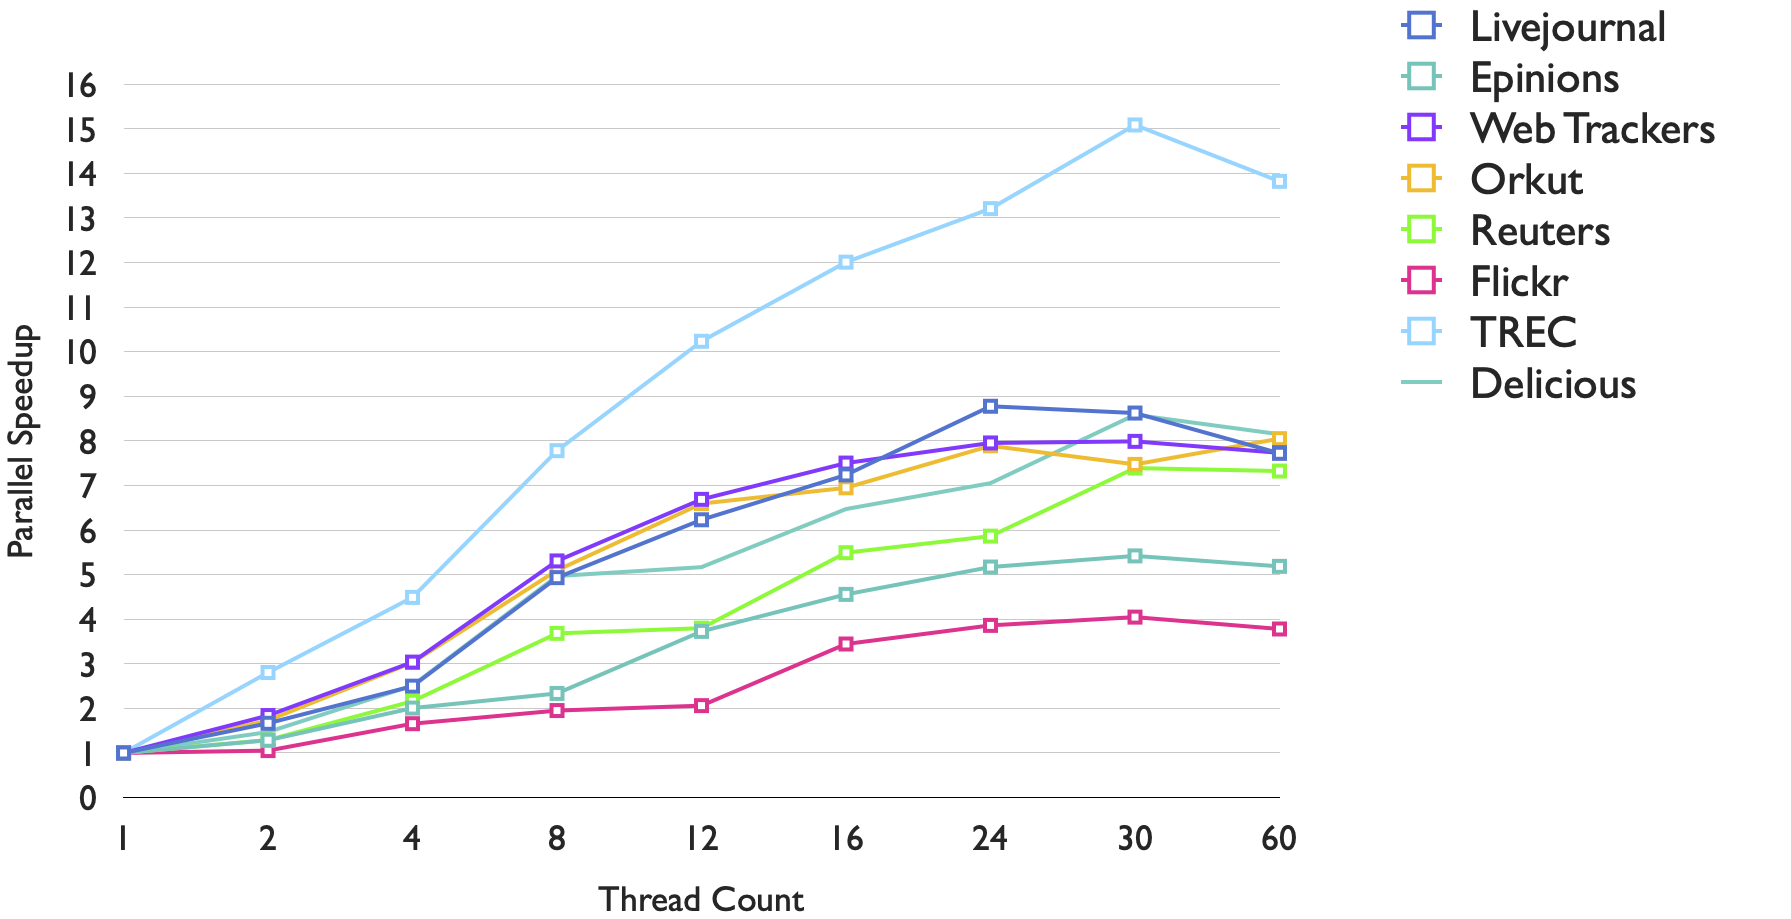
\includegraphics[width=7cm]{figures/speedup-q.png} }}%
    \qquad
    \subfloat[\centering Ratio of runtimes relative to serial time]{{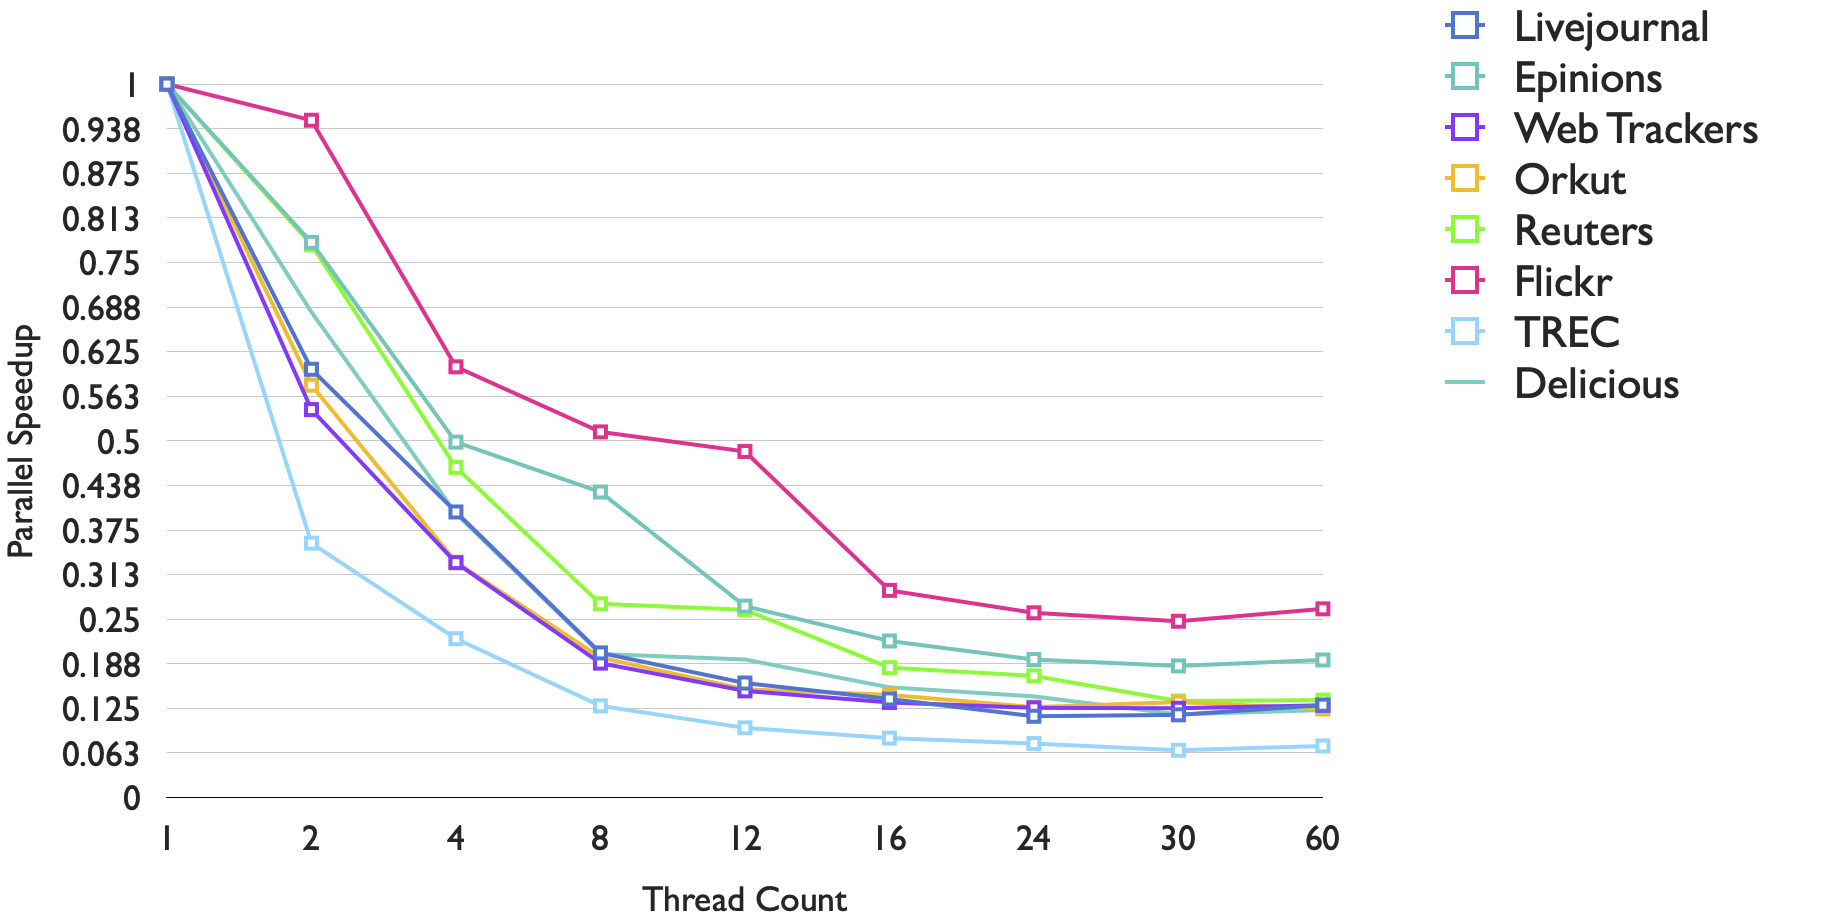
\includegraphics[width=7cm]{figures/runtime-ratio-q.png} }}%
    \caption{Graph (a) shows plots of \algname{par-query}'s speedup over different number of threads used. Graph (b) shows the runtime ratios.}%
    \label{fig:speedup:q}%
\end{figure}

In this section, we give the runtimes of our bi-core index query algorithm. Following the convention adopted by Liu \textit{et al.}, we report the runtime of completing 10 query calls with each query having $\alpha=10,\beta=10$. On the graph Delicious, Liu \textit{et al.} reported a runtime of 0.04 second. \algname{par-query}, running on a single thread, outperforms it, attaining a runtime of 0.0154 second. Our implementation achieves a 2.6x speedup. This proves that our optimization of storing the index structure in CSR format is effective (it potentially reduces the number of cache misses). Using 30 threads, \algname{par-query} achieves a runtime 0.0018 second, which is a 22.3x speedup over the Liu \textit{et al.}'s sequential query algorithm. 

\myparagraph{Analysis of Scalability}

Figure \ref{fig:speedup:q} demonstrates the tangible self-relative speedups achieved by \algname{par-query}. It achieves up to 15.1x self-relative speedup using 30 threads as compared to 1 thread. The speedup achieved is mostly consistent across different graphs, but has higher volatility when compared to the \algname{par-optimized} or \algname{par-index}. This is expected due to the low runtime of the query algorithm as well as its strong dependence on cache efficiency, with parallel copy of contagious array being its only time-consuming operation. 


\section{Conclusion}
In this paper, we study parallel algorithms for bi-core decomposition, which is an important theoretical problem with many real-world applications. We develop the first shared-memory work-efficient parallel bi-core decomposition algorithm with nontrivial span bounds. Our parallel algorithm improves the span complexity from the state-of-the-art $\BigO{m}$ to $\BigO{\rho \log(n)}$ \textit{w.h.p.}. Practically, the span we achieve is 2--3 orders of magnitude lower than the span of existing parallel algorithm. Further, we prove the problem of bi-core decomposition to be P-complete. We also introduce a parallel indexing structure to store the bi-cores, and provide a work-efficient parallel index construction algorithm and query algorithm. Finally, we introduce optimizations such as peeling space pruning and provide optimized implementations of our algorithms. We perform experimental evaluation of our algorithms on real-world bipartite graphs. Our parallel algorithms outperform sequential baselines by up to 44x for peeling and 22.3x for query. Experimental results also prove our bi-core decomposition algorithms are capable of scaling to real-world graphs with hundreds of millions of edges, processing them in minutes and performing bi-core queries in milliseconds. 

% In the future, we hope to further optimize the actual implementation of our algorithm and obtain better runtime results. We also intend to provide a complexity proof to show that the problem of bi-core decomposition is P-complete. We aim to bound the bi-core peeling complexity constant in our span. We also plan to parallelize the index construction and maintenance algorithms introduced Liu \textit{et al.} \cite{Liu2020Efficient}. Moreover, we will perform more comprehensive experiments to demonstrate and analyze the performance of our algorithms. As extension to the work on bi-core, we may also investigate parallel bi-clique peeling or parallel community search in bipartite graphs. 

\section*{Acknowledgements}

We would like to thank Jessica Shi and Professor Julian Shun (MIT CSAIL) for their amazing support and guidance throughout the year. In addition, we thank the MIT PRIMES organization for this opportunity. 

\bibliographystyle{ACM-Reference-Format}
\bibliography{references}

\end{document}
